
%\section{Supplementary Information}
\chapter{Supplementary figures for Comparison of non-local sequence-dependent mechanics of DNA in protein-DNA crystal structures ensemble with cgNA$+$ model}\label[appendix]{app5}

\section{Additional figures and tables}

% \begin{figure}[H]
% 	\begin{center}
% 	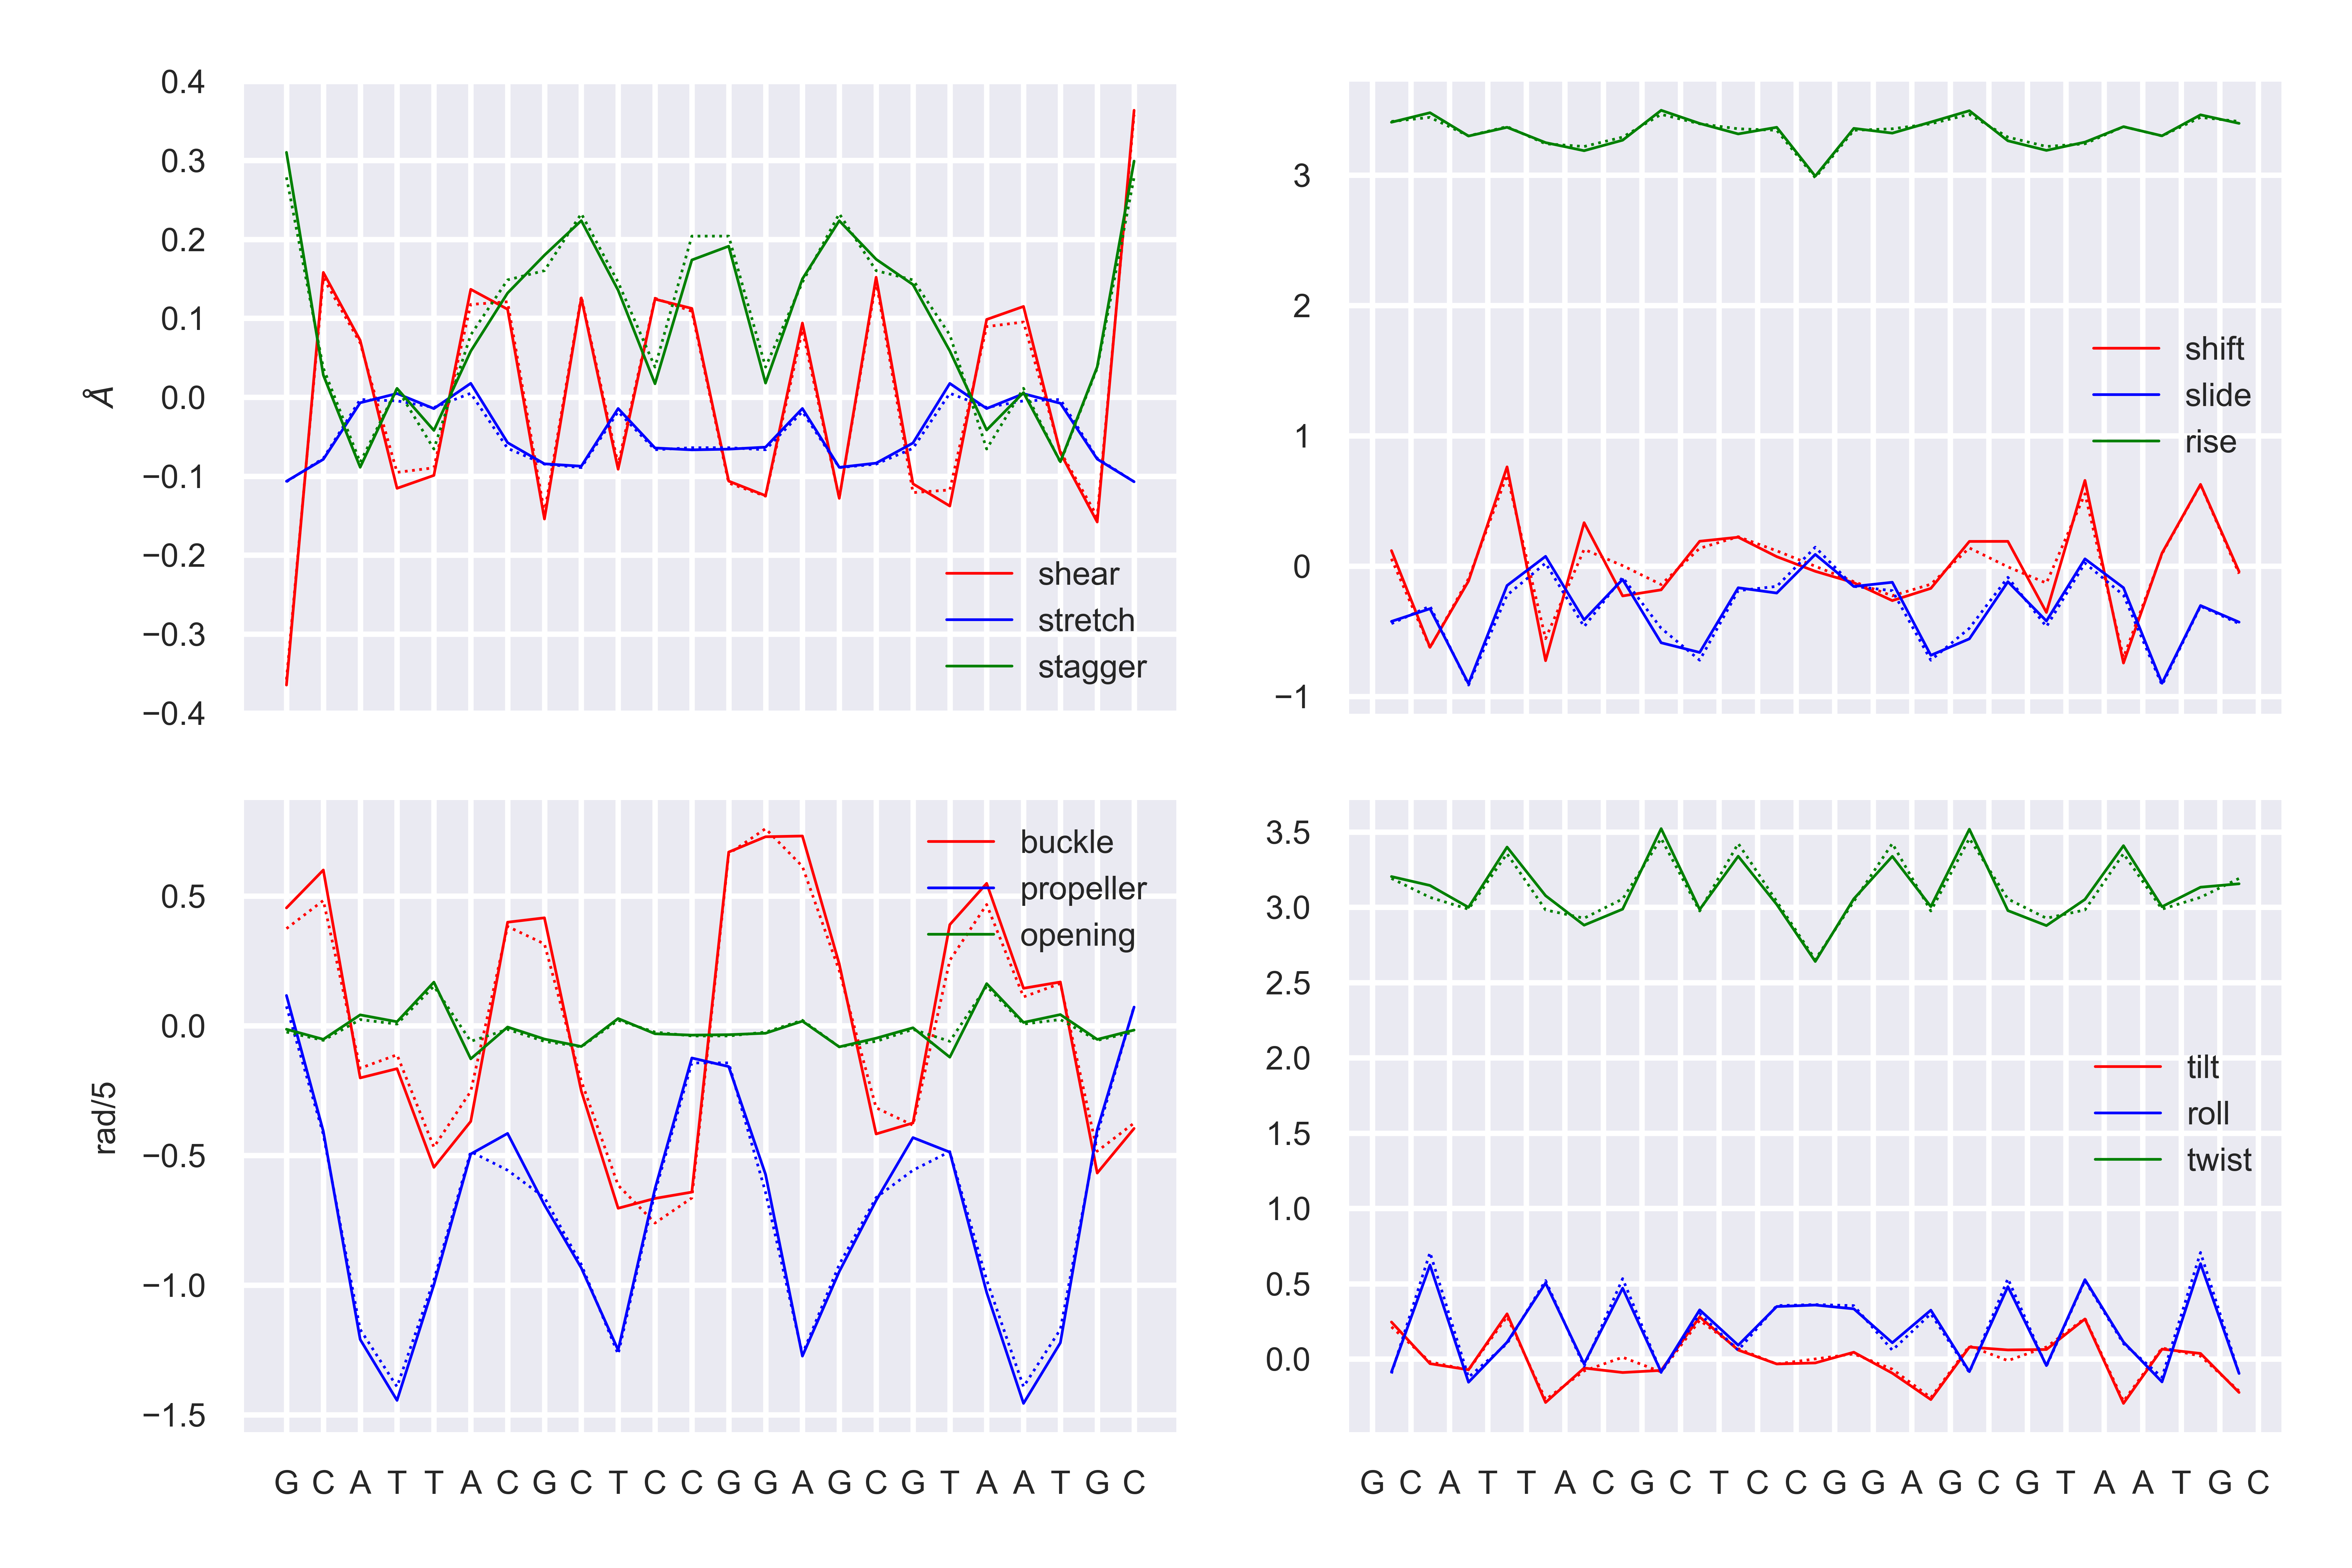
\includegraphics[scale=1]{./Xray_images/dna_cg_recons_error_mu_seq_17.png}
% 	\caption{The groundstate predicted by cgNA$+$ model for a sequence  `GCATTACGCTCCGGAGCGTAATGC' (note that the sequence is outside the training library for cgNA$+$ model) is plotted in solid lines (------) and the corresponding atomistic MD groundstate is plotted in $\cdots$.
% 	}
% \label{SIfig:testerror}
% \end{center}
% \end{figure}

% \begin{figure}[H]
% 	\begin{center}
% 	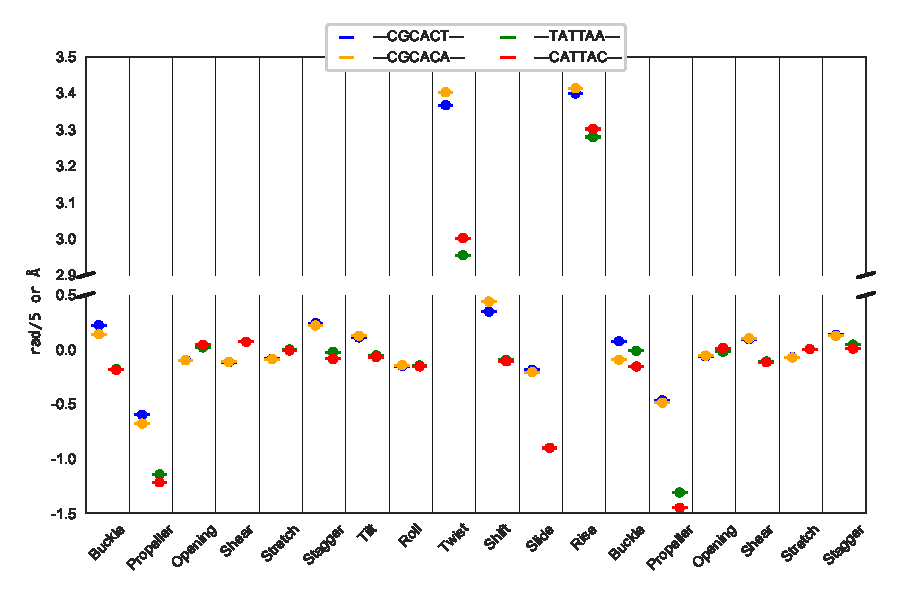
\includegraphics[scale=1]{./Xray_images/hex_context_effect.pdf}
% 	\caption{Internal coordinates of middle-junction dimer of tetramer in different beyond tetramer context highlighting the sequence effect on groundstate of dimer due to beyond tetramer context.
% 	The $\bullet$ is MD simulations data and $-$ is cgNA$+$ predictions and the two data sets are indistinguishable. Note that beyond hexamer context is also different but concisely represented by \,-\,-\,-\,.
% 	}
% \label{SIfig:hex_context1}
% \end{center}
% \end{figure}


\begin{figure}[H]
	\begin{center}
	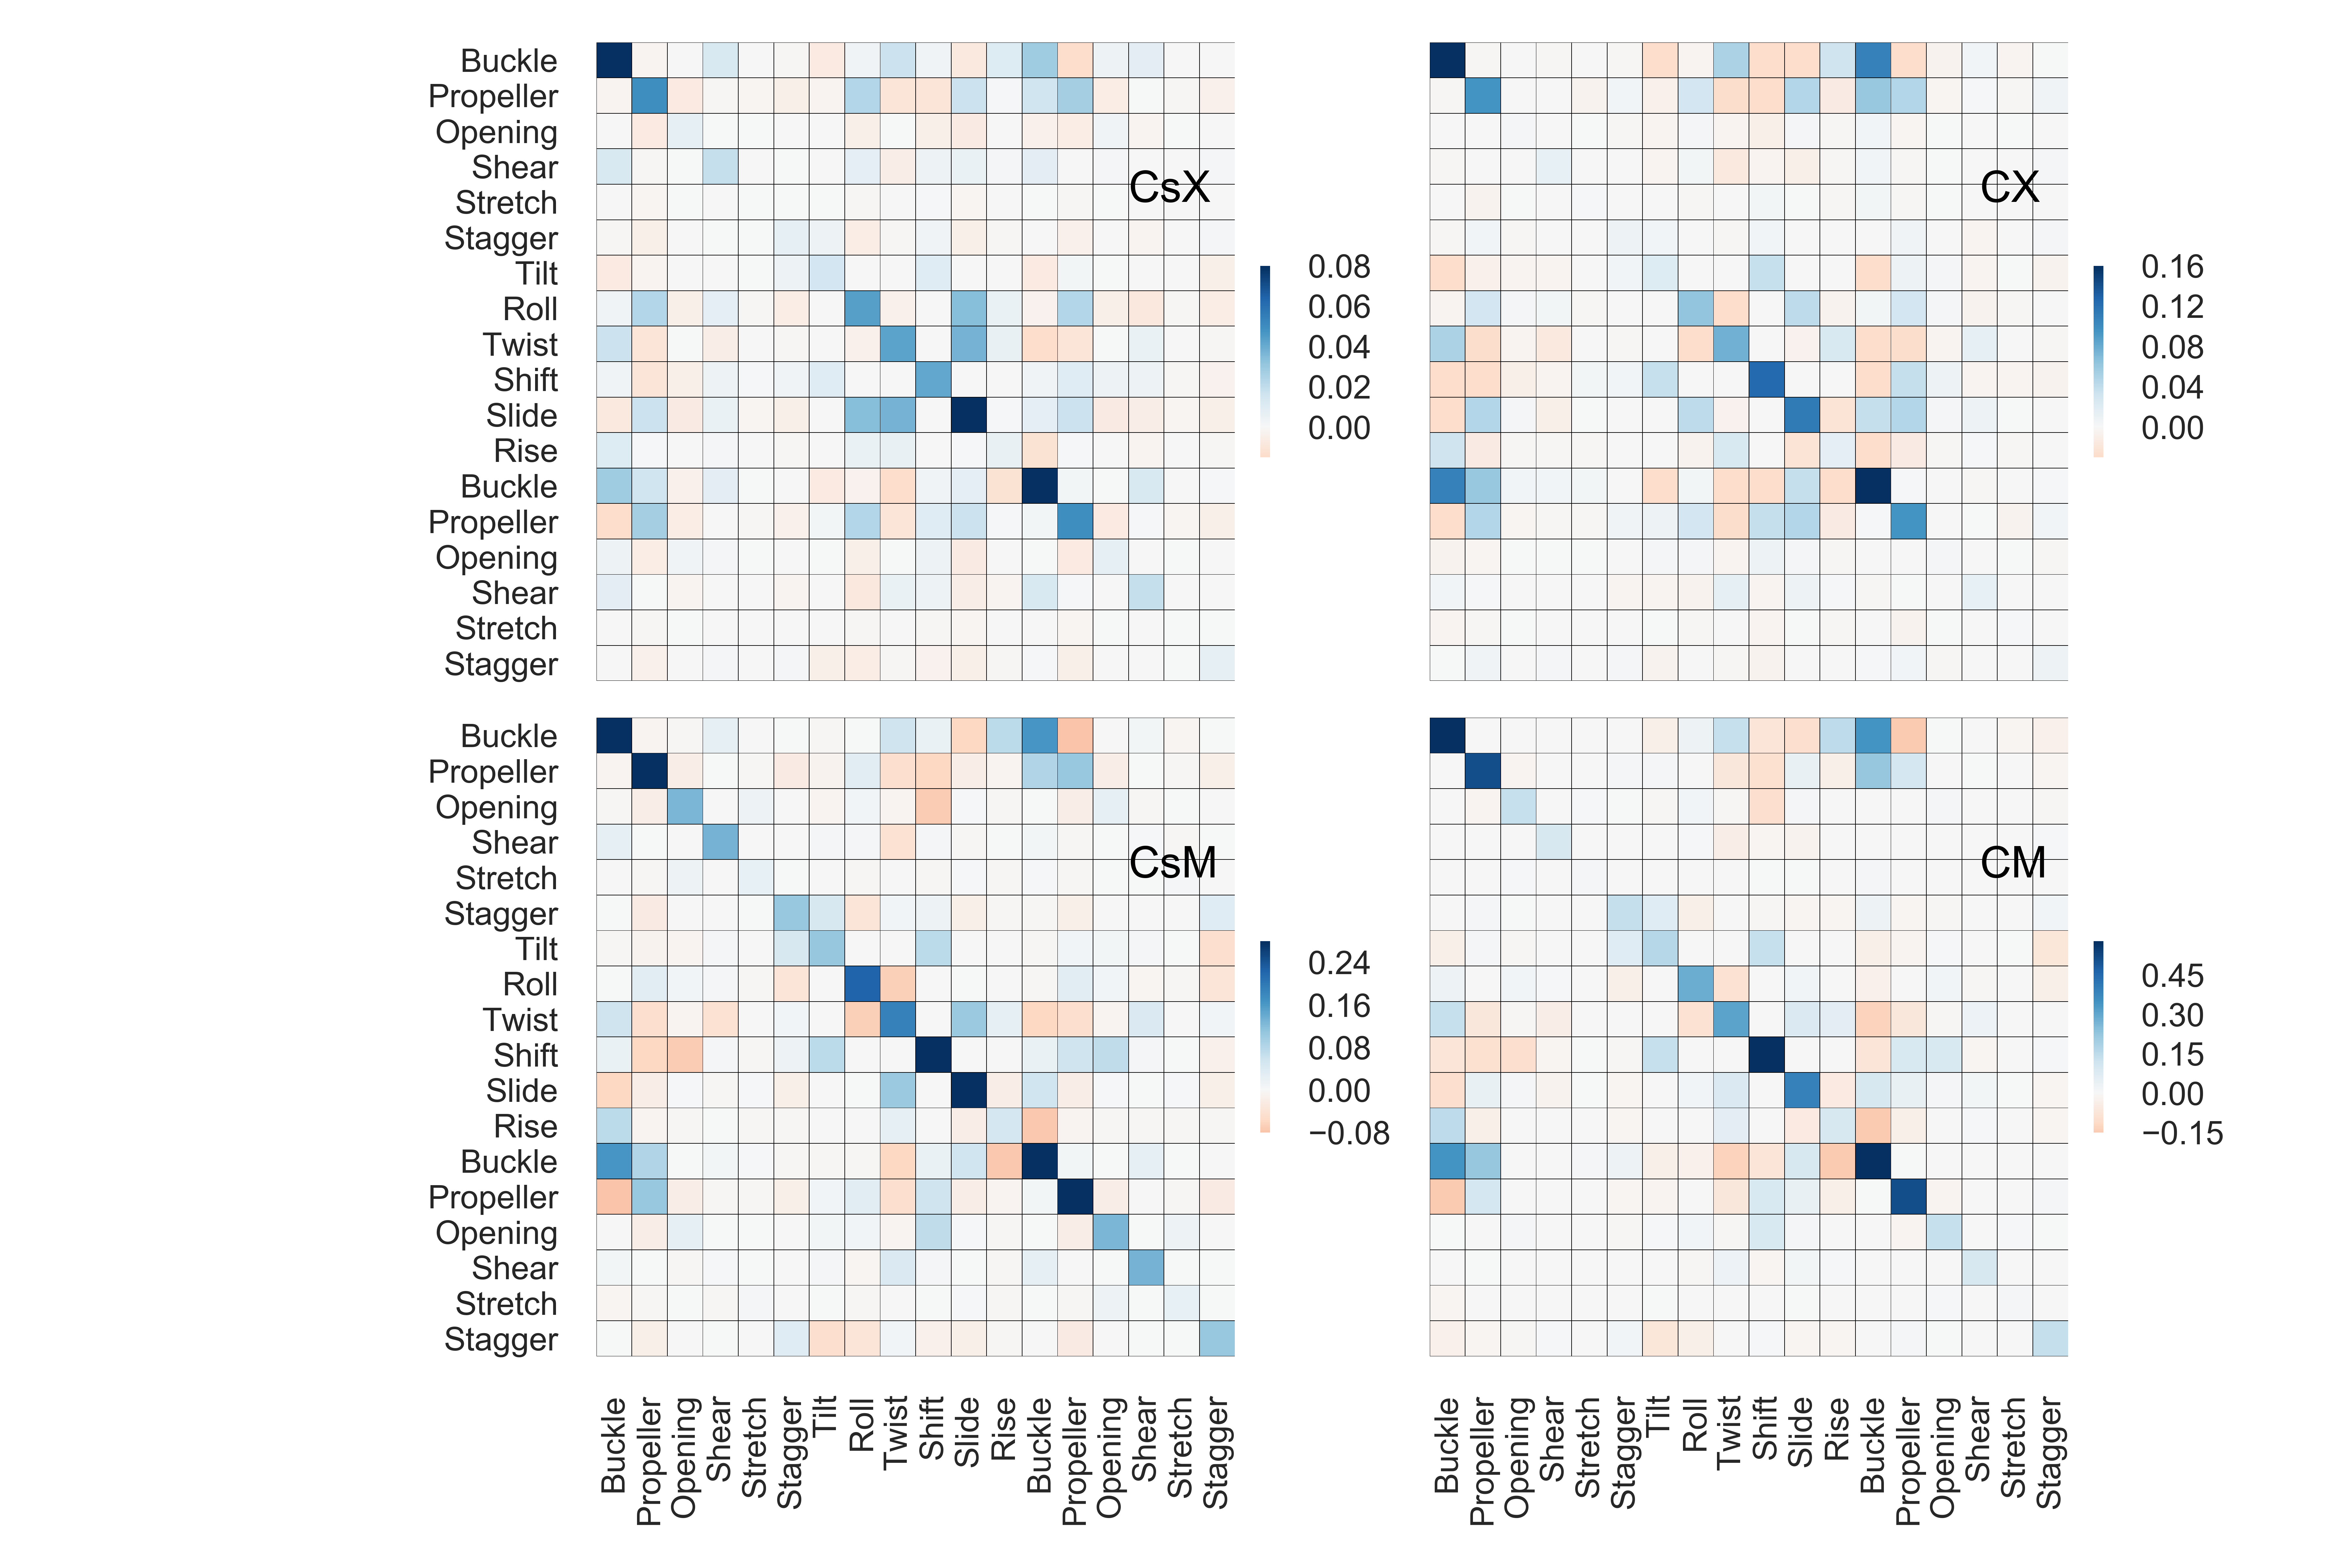
\includegraphics[scale=1]{./Xray_images/C_4.png}
	\caption{Heat map for shape and configuration covariance for X-ray ($C_sX$ and $CX$) and cgNA$+$ ($C_sM$ and $CM$) model data set. The corresponding variances are listed in the \cref{tab:var_table}. Note that the scale in all four covariance is different. Scale of configuration covariance is approximately two times that shape covariance in both the data set. Scale in cgNA$+$ model data set, for both the covariance (shape and configuration), is almost three times than in X-ray data set possibly due less effective temperature in X-ray data set.  
	}
\label{SIfig:cov_4}
\end{center}
\end{figure}


\begin{table}[H]
\begin{tabular}{ccccc}
Internal  & Shape  & Shape  & Configurational  & Configurational \\
 Coordinate &  variance (X-ray) & variance (CG) &  variance (X-ray) &  variance (CG) \\
\hline
\hline
Buckle & 0.0799 & 0.2441 & 0.4764 & 0.9488 \\
Propeller & 0.0499 & 0.0956 & 0.3487 & 0.5143 \\
Opening & \textbf{0.0070} & 0.0035 & 0.1272 & 0.1335 \\
Shear & 0.0191 & 0.0136 & 0.1333 & 0.0954 \\
Stretch & \textbf{0.0006} & 0.0013 & 0.0231 & 0.0136 \\
Stagger &  \textbf{0.0073} & 0.0092 &  0.1061 &  0.1361 \\
\hline
Tilt & 0.0147 &  0.0223 & 0.1078 & 0.1660  \\
Roll &  0.0439 &  0.0629 &  0.2241 &  0.2870  \\
Twist &  0.0432  &  0.0767  &   0.1888 & 0.3094 \\
Shift & 0.0413  & 0.1238  & 0.3470  &  0.6836  \\
Slide &  0.1447 &  0.1127  &  0.4347 & 0.3938  \\
Rise  & \textbf{0.0063}   & 0.0167  &  0.0497  &    0.0964 

\end{tabular}
\caption{List of variances (the diagonal elements) for shape and configuration covariances for X-ray and cgNA$+$ model data set. The unit for the variance can be considered as $\text{\AA}^2$  and $(\text{rad}/5)^2$ for 
translational and rotational coordinates, respectively. The corresponding full covariance matrix is plotted in \cref{SIfig:cov_4}. Due to palindromic symmetry, the variance for both the base-pairs (in terms of intra coordinates) is identical and, thus, listed once. 
}
\label{tab:var_table}
\end{table}


\begin{figure}[H]
	\begin{center}
	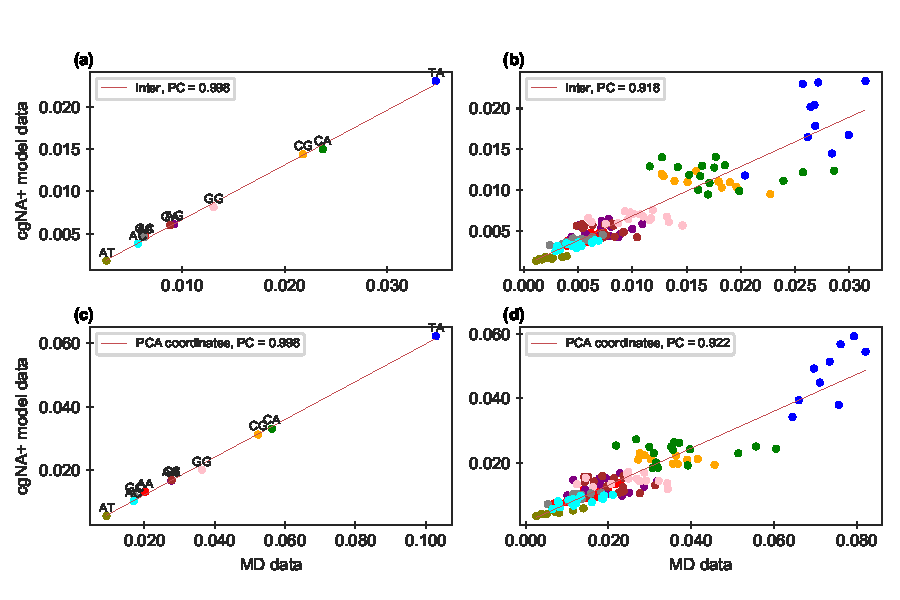
\includegraphics[scale=1]{./Xray_images/vol_R2_CG-MD.pdf}
	\caption{Comparison of configurational volume (S)
	for cgNA$+$ model covariance vs MD data set covariance a) in inter coordinates for independent dimer steps in average context, b) in inter coordinates for dimers in independent tetramer contexts, c) in PCA coordinates (in  eight principal modes of cgNA$+$ model shape covariance) for independent dimer steps in average context, d) in PCA coordinates (in  eight principal modes of cgNA$+$ model shape covariance) for dimers in independent tetramer contexts.
	The red line is best-fit line between the two data sets using linear regression.}
\label{SIfig:MDstiff}
\end{center}
\end{figure}


\begin{figure}[H]
	\begin{center}
	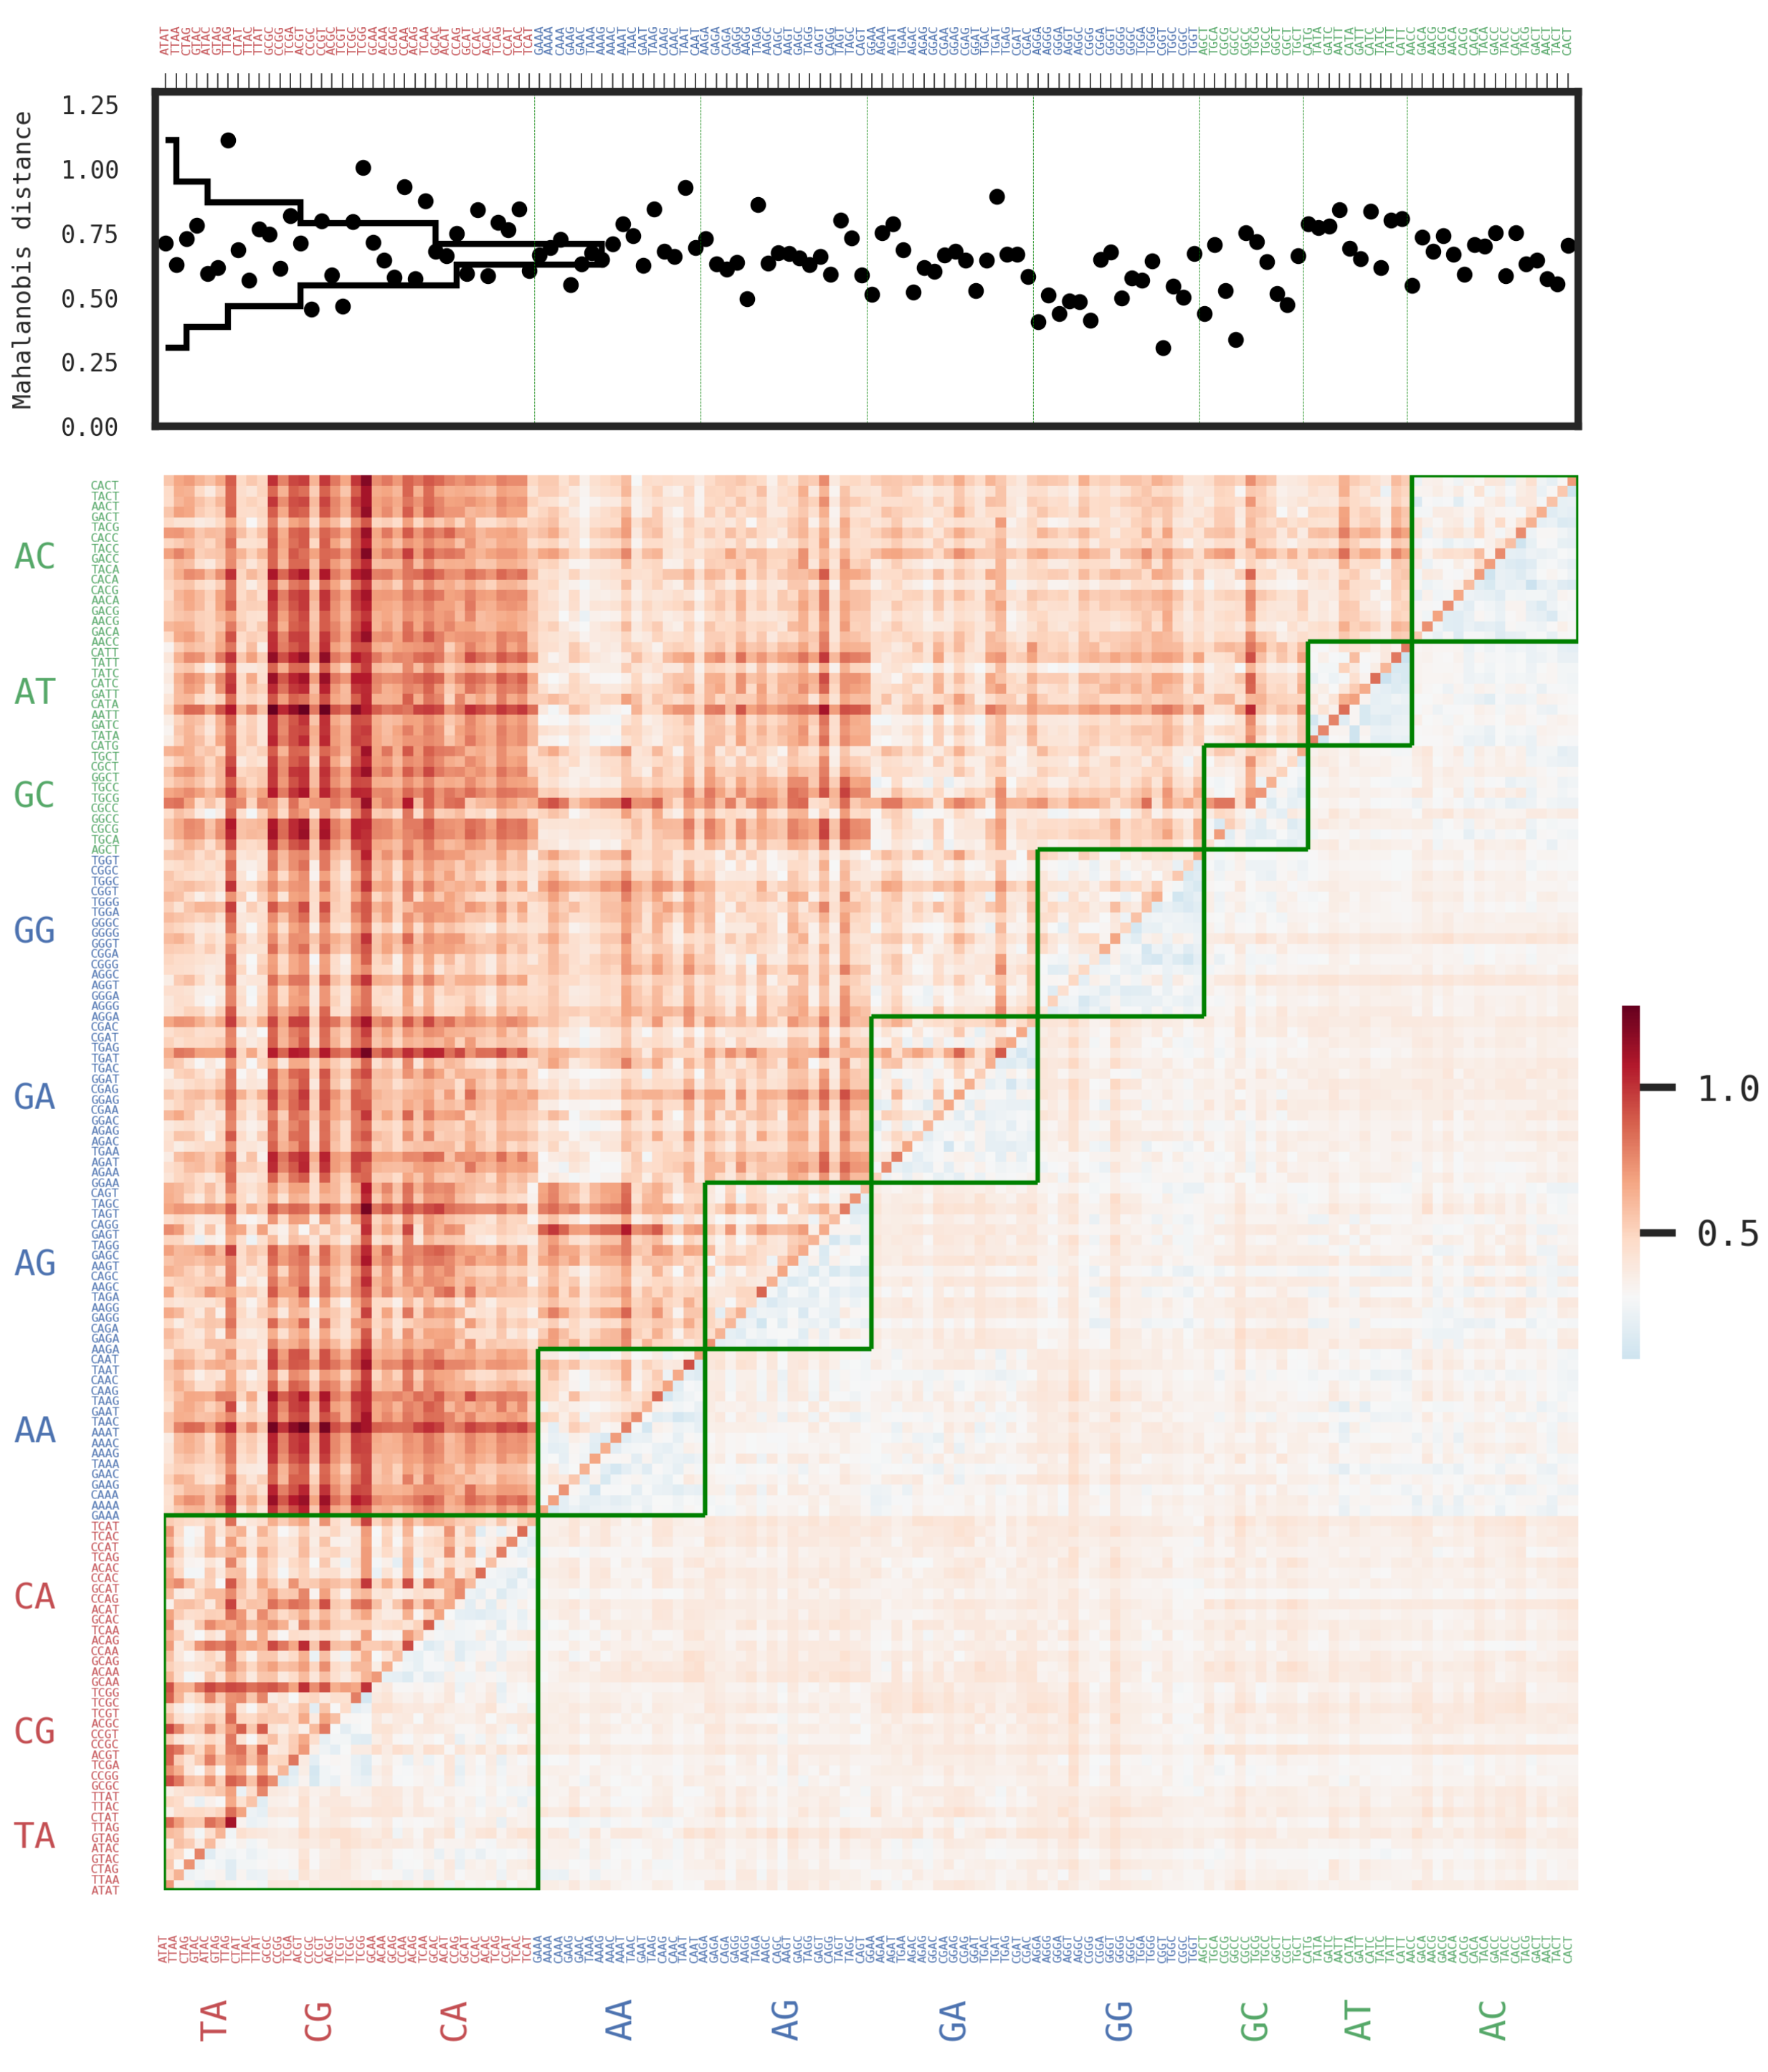
\includegraphics[scale=1.45]{./Xray_images/X3_heat_mahal_pca_18_comb.png}
	\caption{
	The diagonal entries in the heat map (bottom) are Mahalanobis distance between the groundstate of dimers (in 136 independent tetramer contexts) in the X-ray and cgNA$+$ model data set. Whereas lower and upper off-diagonal entries are Mahalanobis distance between different dimers (in specific tetramer context) within the cgNA$+$ model and X-ray data set, respectively. The diagonal entries of the heat-map are again plotted in the scatter plot (top) along with the histogram in the same plot.
	Note that the Mahalanobis distance (as defined in \cref{eq:mahal_eq}) is computed in the 18 CURVES$+$ coordinates and using the cgNA$+$ shape covariance matrix as the weight matrix. 
    }
\label{SIfig:Mahal_18}
\end{center}
\end{figure}


% \begin{figure}[H]
% 	\begin{center}
% 	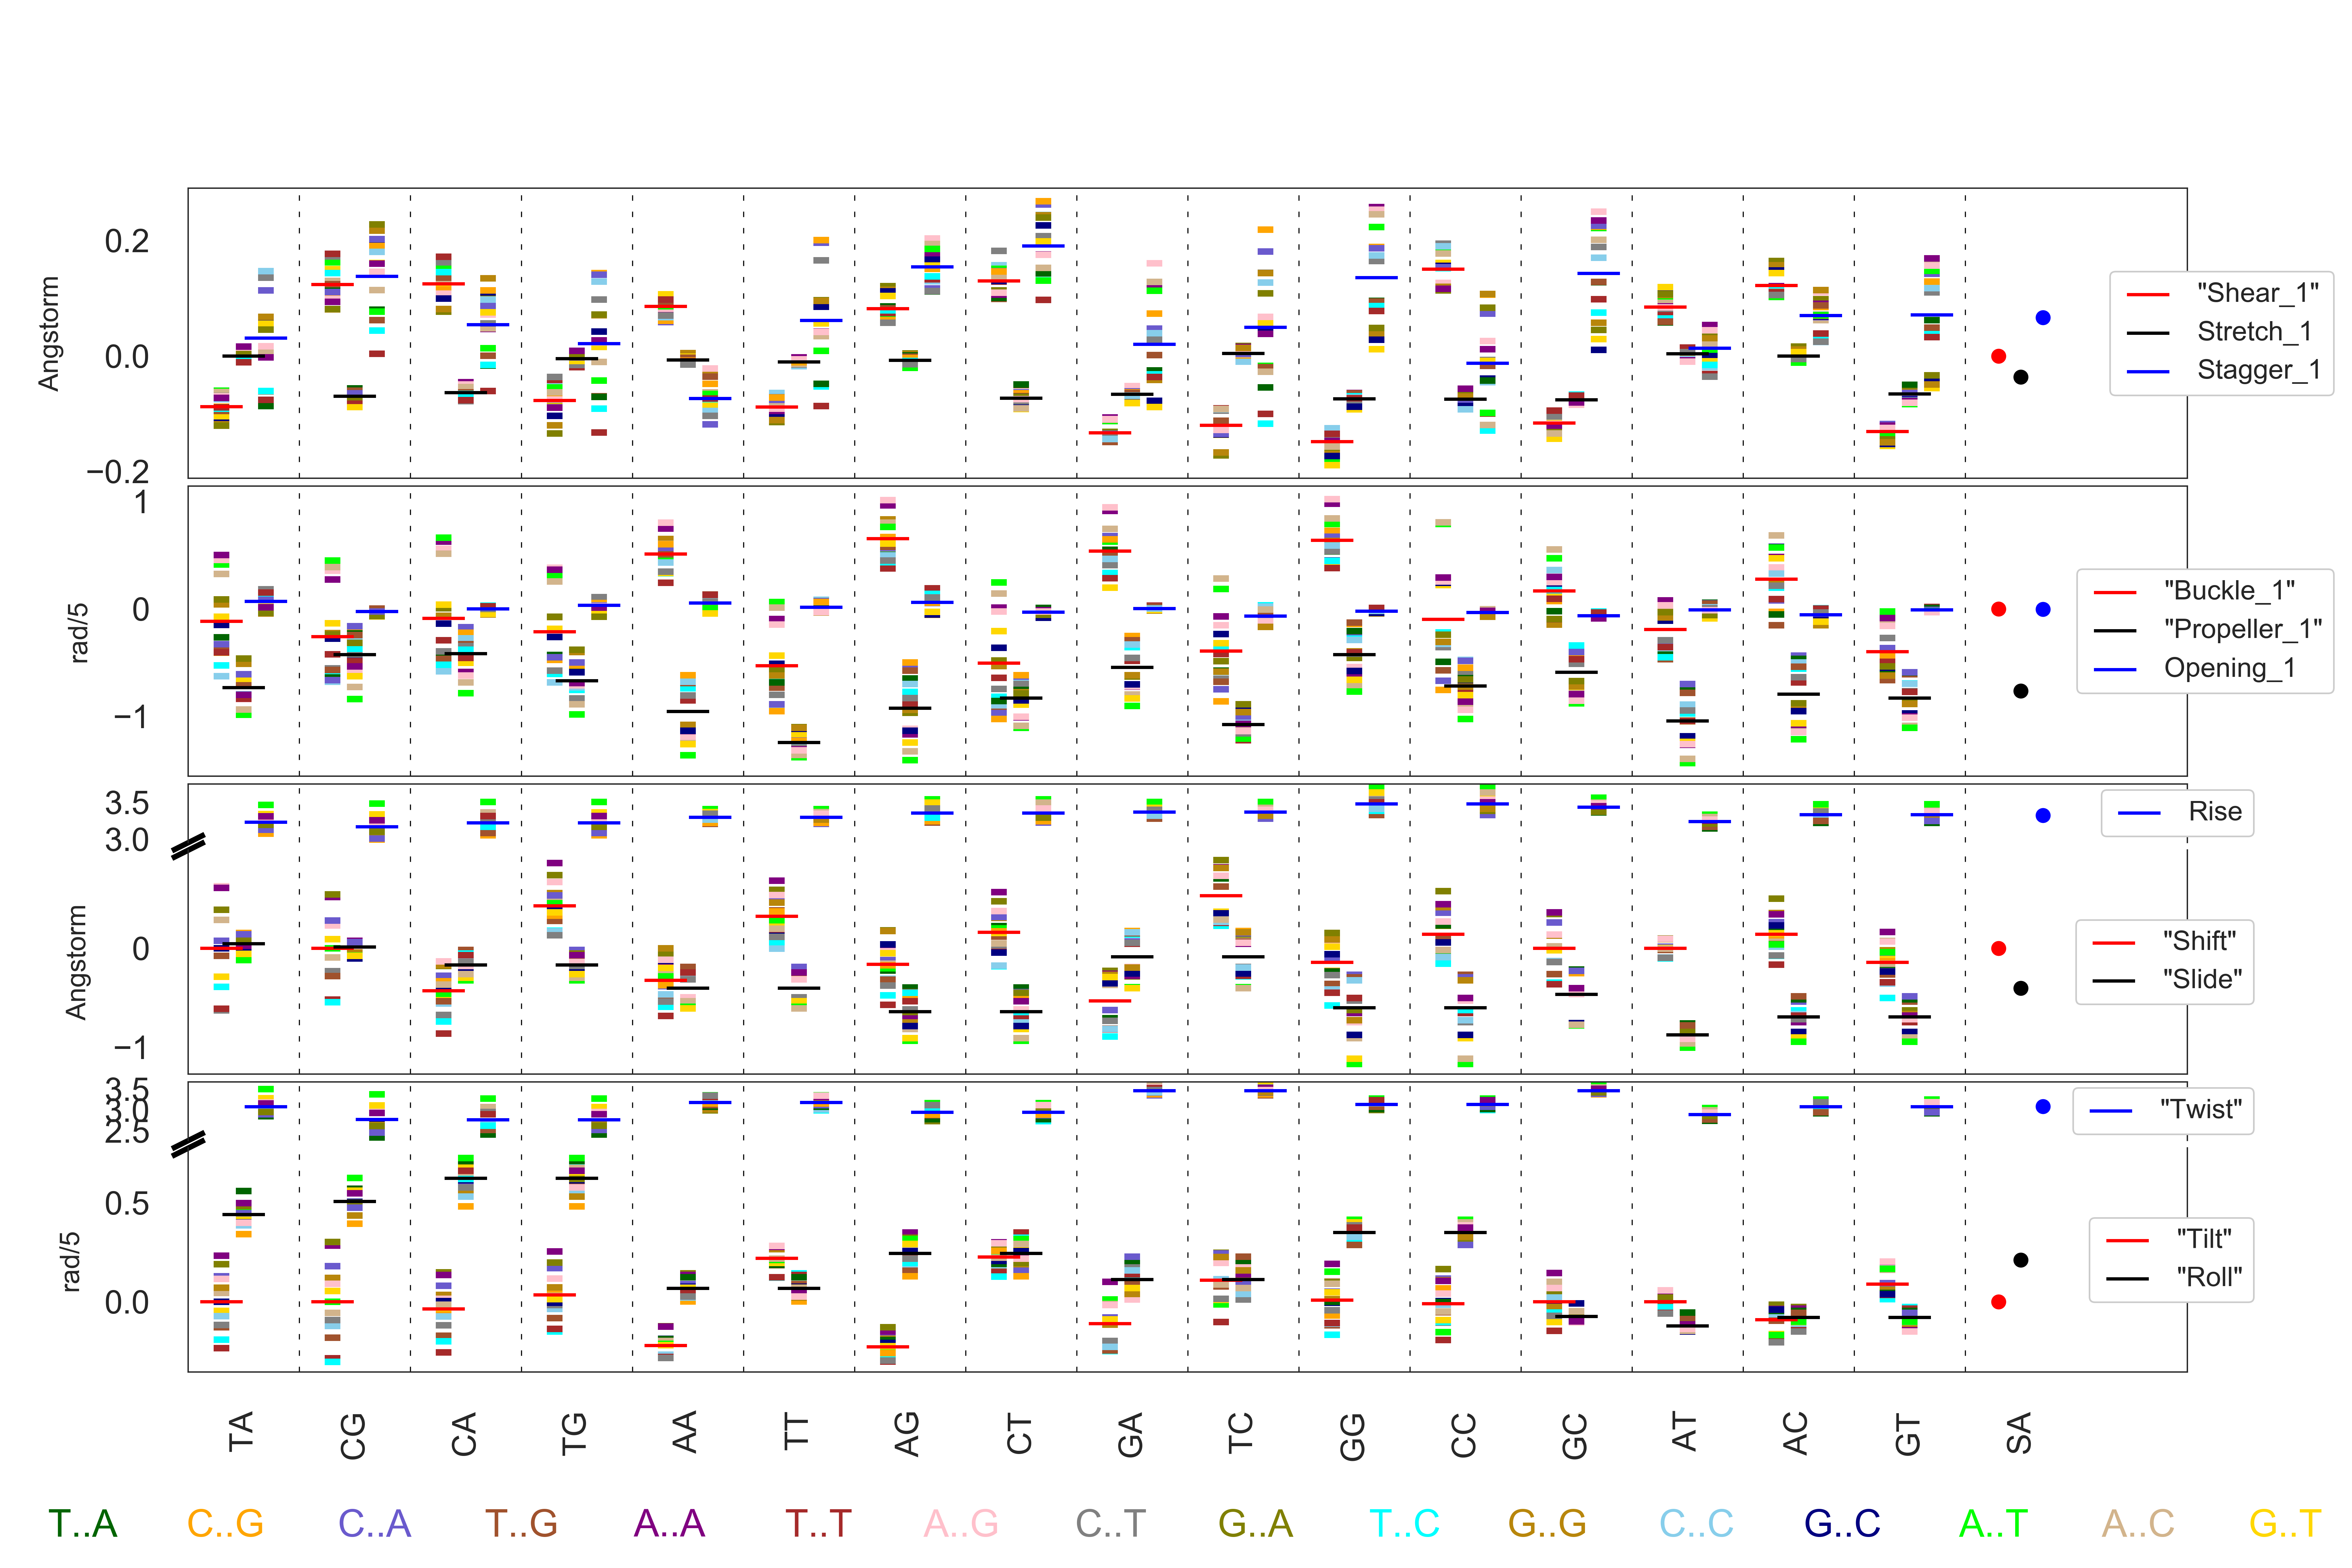
\includegraphics[scale=1]{./Xray_images/seq_var_comb_256_cgDNA.png}
% 	\caption{Plot of Intras and Inter for cgNA$+$ model data set where large dash line plots the internal coordinate of a dimer (in average context) while the other smaller dash lines are the values of internal coordinates for that dimer in its specific tetramer context. For better and concise visual representation, in each subplot, the three IC are slightly shifted on the X-axis. Also, separate flanking context is plotted in different color as described on the bottom of the plot. SA is sequence average groundstate. 
% 	}
% \label{SIfig:seq_imp2}
% \end{center}
% \end{figure}



%\begin{figure}[H]
%	\begin{center}
%	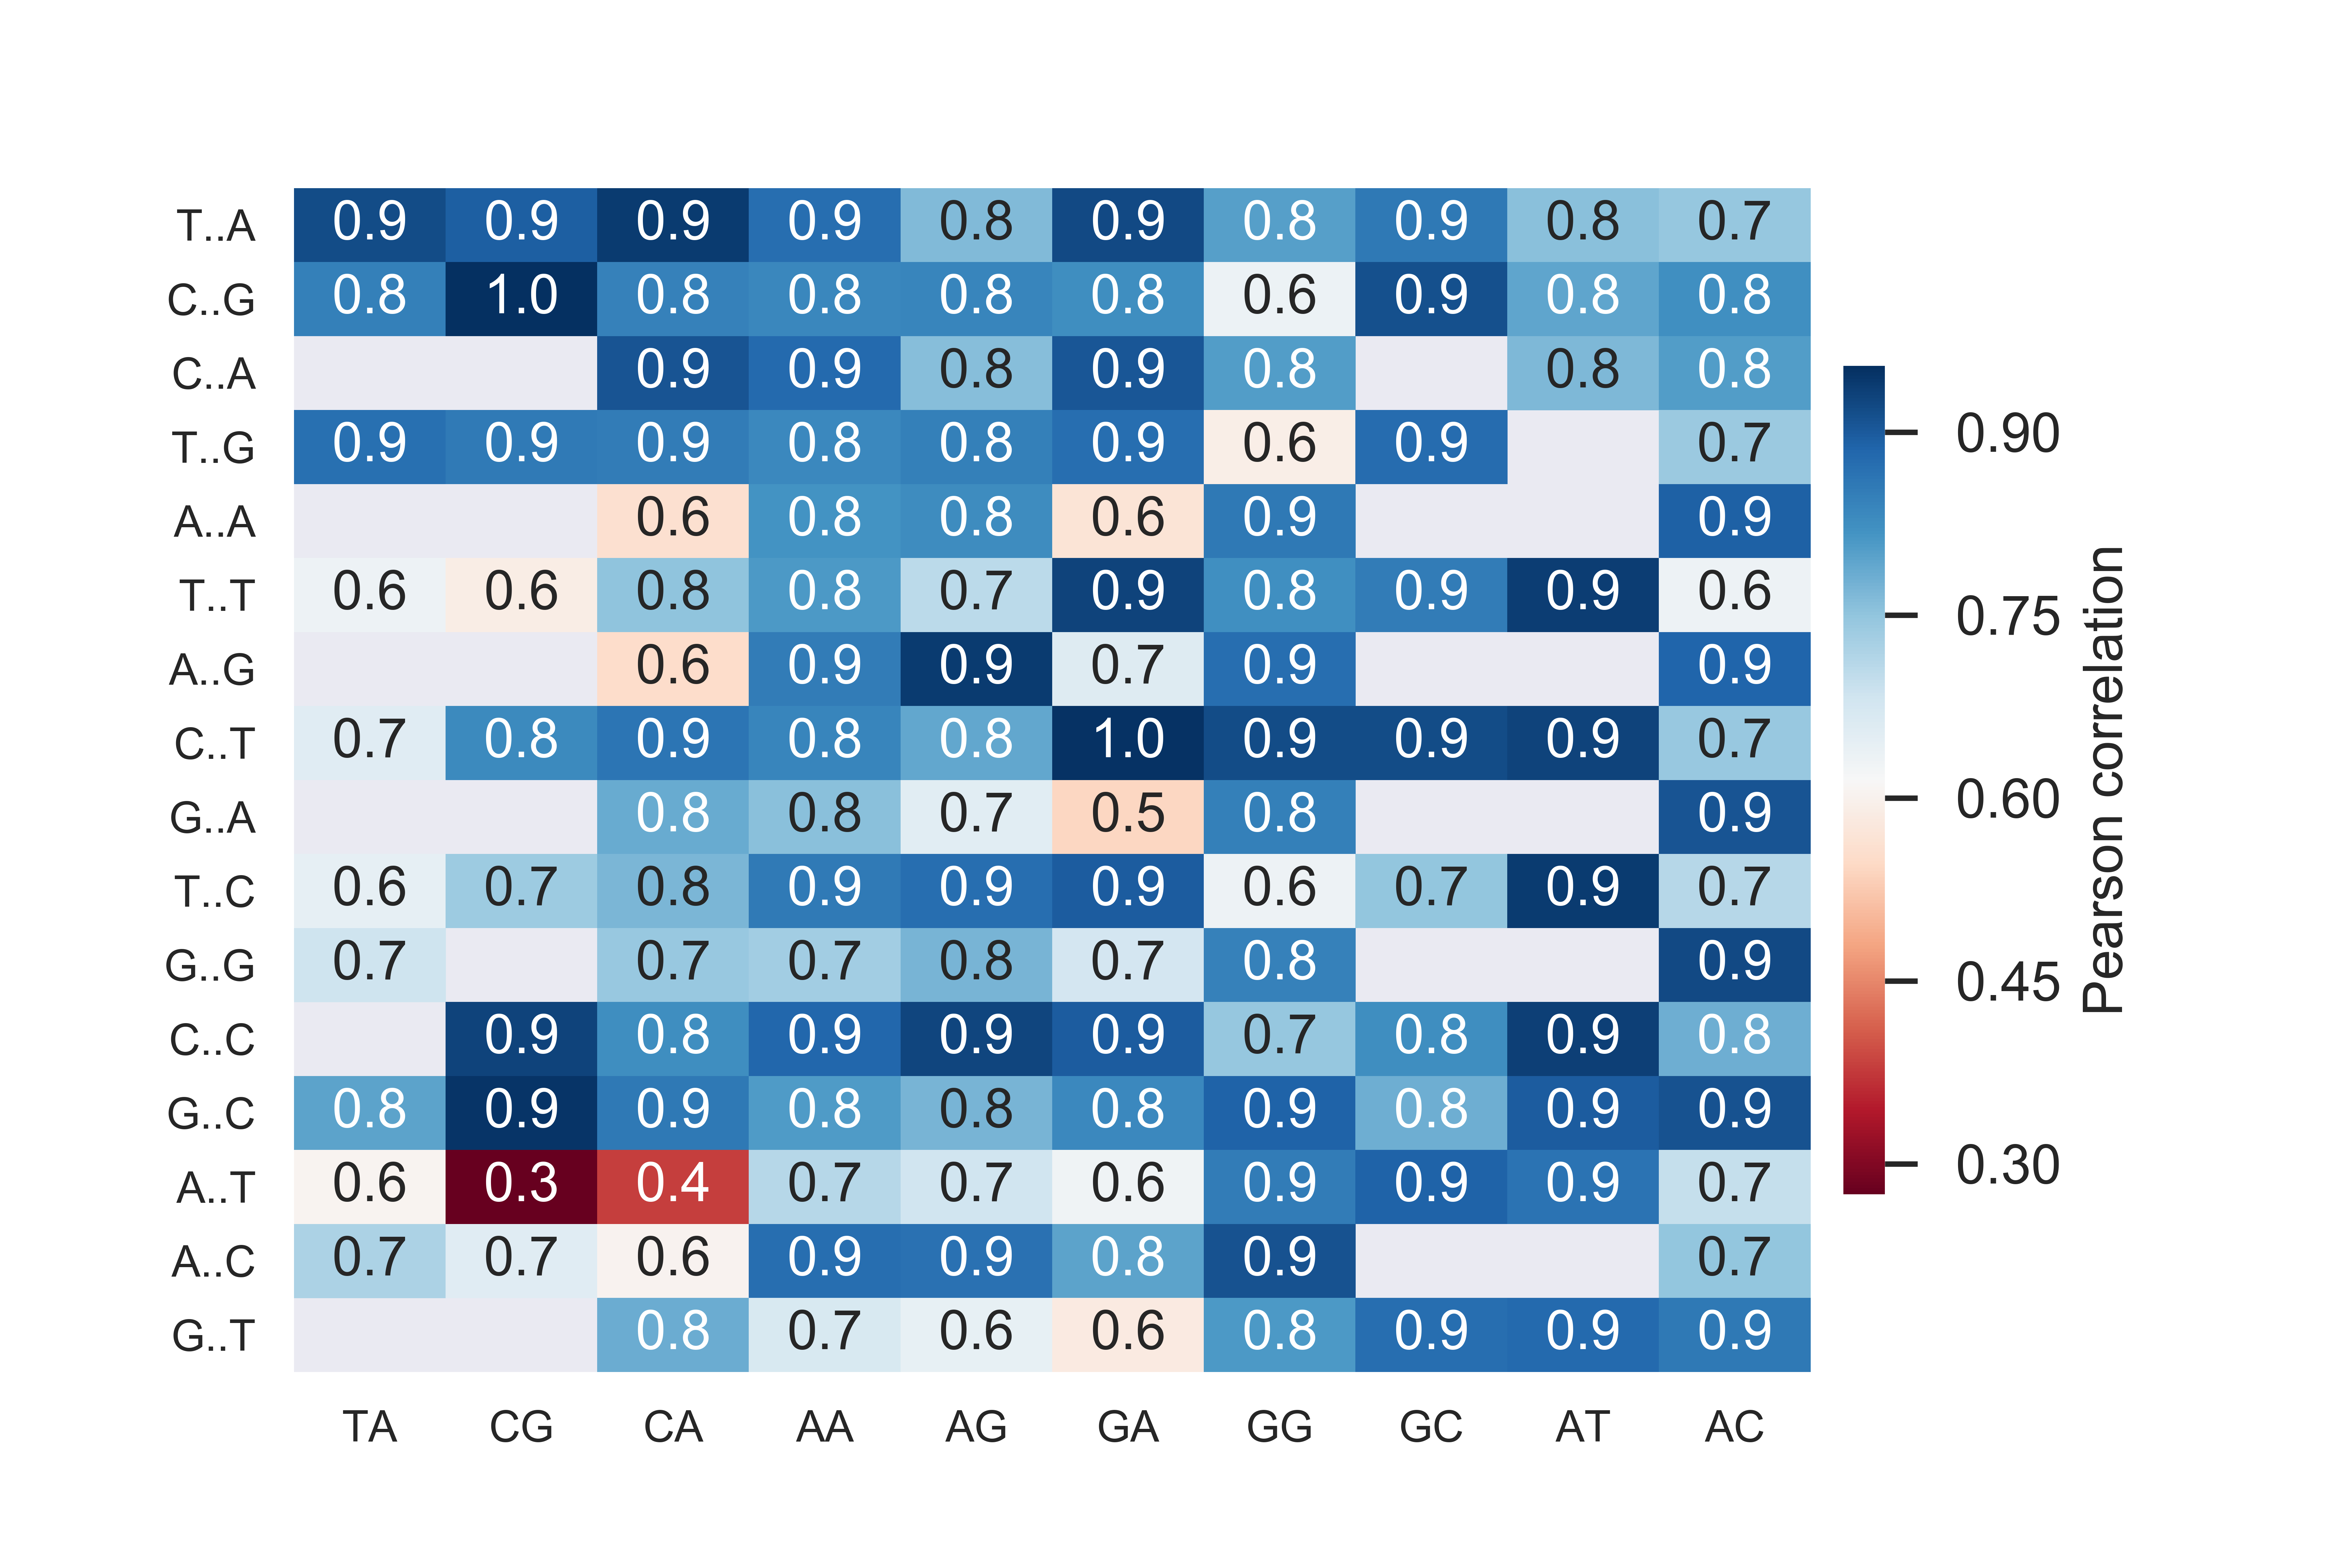
\includegraphics[scale=1]{./Xray_images/seq_var_heat_map_CG.png}
%	\caption{Difference in terms of linear correlation for dimer (in avg. flanking sequence ) with dimer in specific tetramer context in cgNA$+$ model data set.  Abscissa is middle junction dimer-step and ordinate is tetramer context. The blank entries in the plot represent the dependent tetramer.
%	}
%\label{SIfig:seq_var_heatmap_CG}
%\end{center}
%\end{figure}



%\section{Influence on environmental conditions on internal coordinates of DNA}
%In order to investigate the influence of 
%salt-type or its concentration, we have performed $3 \mus$ MD simulations for two sequences, GCTAATCGGTGCGC and GCGACAGCCTTAGC, using the same MD protocol as used for cgNA$+$ training library.  
%We performed 10 sets of simulations for 5 different salt concentration (20, 50, 100, 250, 500 mM) and two different salt types (KCl and Nacl). 
%In \cref{SIfig:ion_effect}, we have plotted 
%the change in IC (phosphates, and inter and intra base-pair coordinates) at dimer-level due to change in concentration of NaCl and KCl salt in blue and red, respectively while the change due to change in salt-type is plotted in green. As can be seen from the plot, the influence of environmental conditions on phosphates is much higher that intra and inter base-pair coordinates.  
%For example, the standard deviation in phosphates rotational and translational coordinates on changing the concentration of NaCl is $\sim 3.25$ and $\sim 6$ times than in intra base-pair coordinates.

%\begin{figure}[H]
%	\begin{center}
%	\includegraphics[scale=1]{./Xray_images/ion_effect.png}
%	\caption{ phos 
%	}
%\label{SIfig:ion_effect}
%\end{center}
%\end{figure}





%\subsection{Results for case-\Rom{2} data}
%In this section, we have plotted the analogous results as in the main chapter but for the X-ray data 
% \begin{figure}[H]
% 	\begin{center}
% 	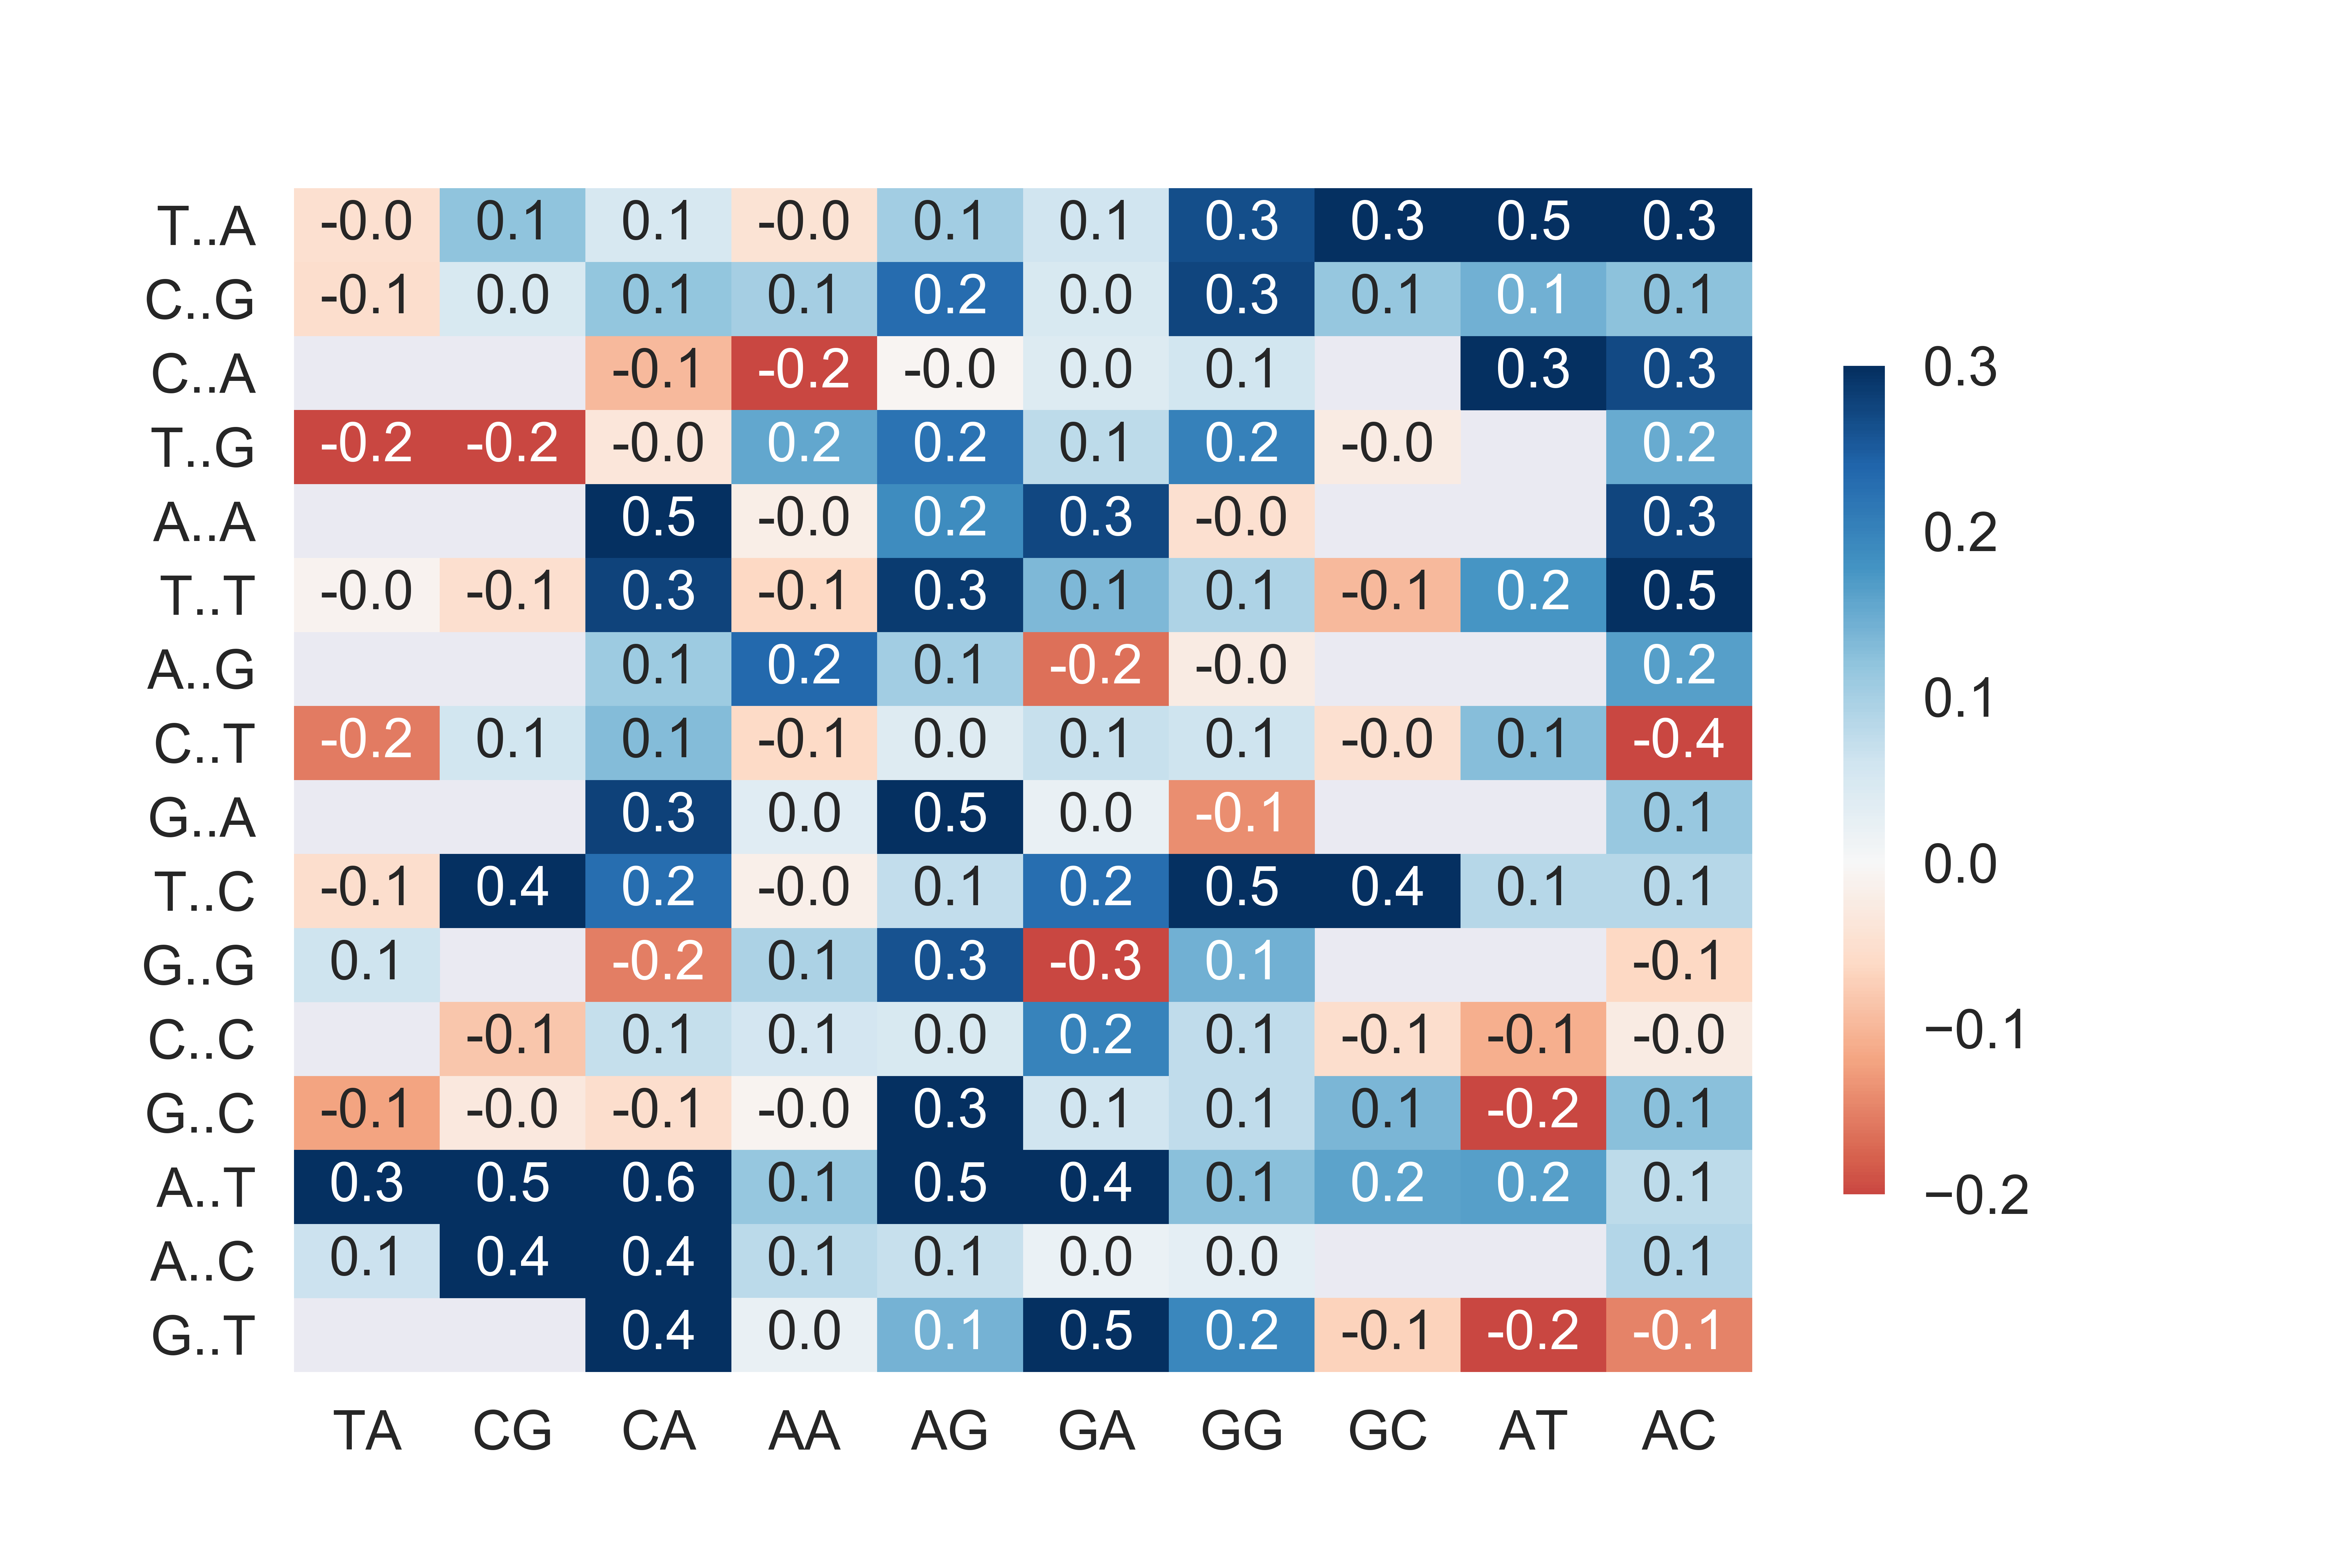
\includegraphics[scale=1]{./Xray_images/heat_map_TX2_PC_imprv.png}
% 	\caption{Heat-map plotting the improvement in linear correlation 
% 	while predicting  X-ray dimer groundstate in tetramer context by cgNA$+$ dimer in tetramer context and cgNA$+$ dimer in average flanking sequence.
%  Abscissa is middle junction dimer-step and ordinate is tetramer context. The blank entries in the plot represent the dependent tetramer.	}
% \label{SIfig:model_comp}
% \end{center}
% \end{figure}


\begin{figure}[H]
	\begin{center}
	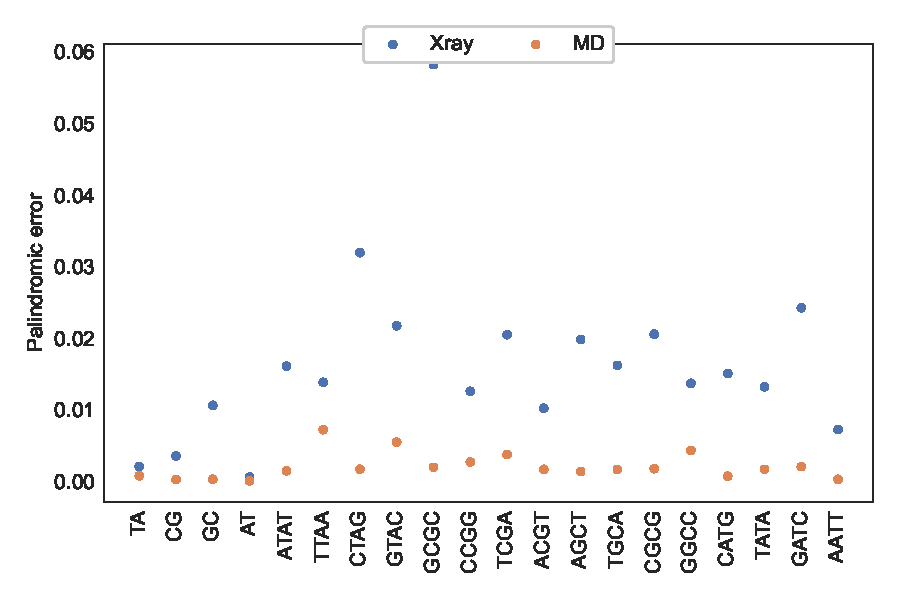
\includegraphics[scale=0.8]{./Xray_images/palin_err_tt3_3S_C1_cg_unsym.pdf}
	\caption{
    Palindromic error (as defined in \cref{c2:s5sb1}) per degree of freedom in the groundstate of palindromic dimer in tetramer flanking context and in average flanking context for X-ray data set and MD simulations (used to train cgNA$+$ model). 
%    As described in \cref{ss:parity}, groundstate ($\mu$) for palindromic dimer should be invariant of the reading strand which allows us to define the palindromic error as $|\mu-E\mu|$ to quantify the convergence of groundstate where $E$ is reading strand transformation matrix defined in \cref{SIeq:Ematint}. 
    %Even though the palindromic error is a norm of a vector with mixed rotational and translational entries, the length scale of palindromic error can be treated in \AA \; or rad/5 units.
	}
\label{SIfig:palin_error}
\end{center}
\end{figure}



% \begin{figure}[H]
% 	\begin{center}
% 	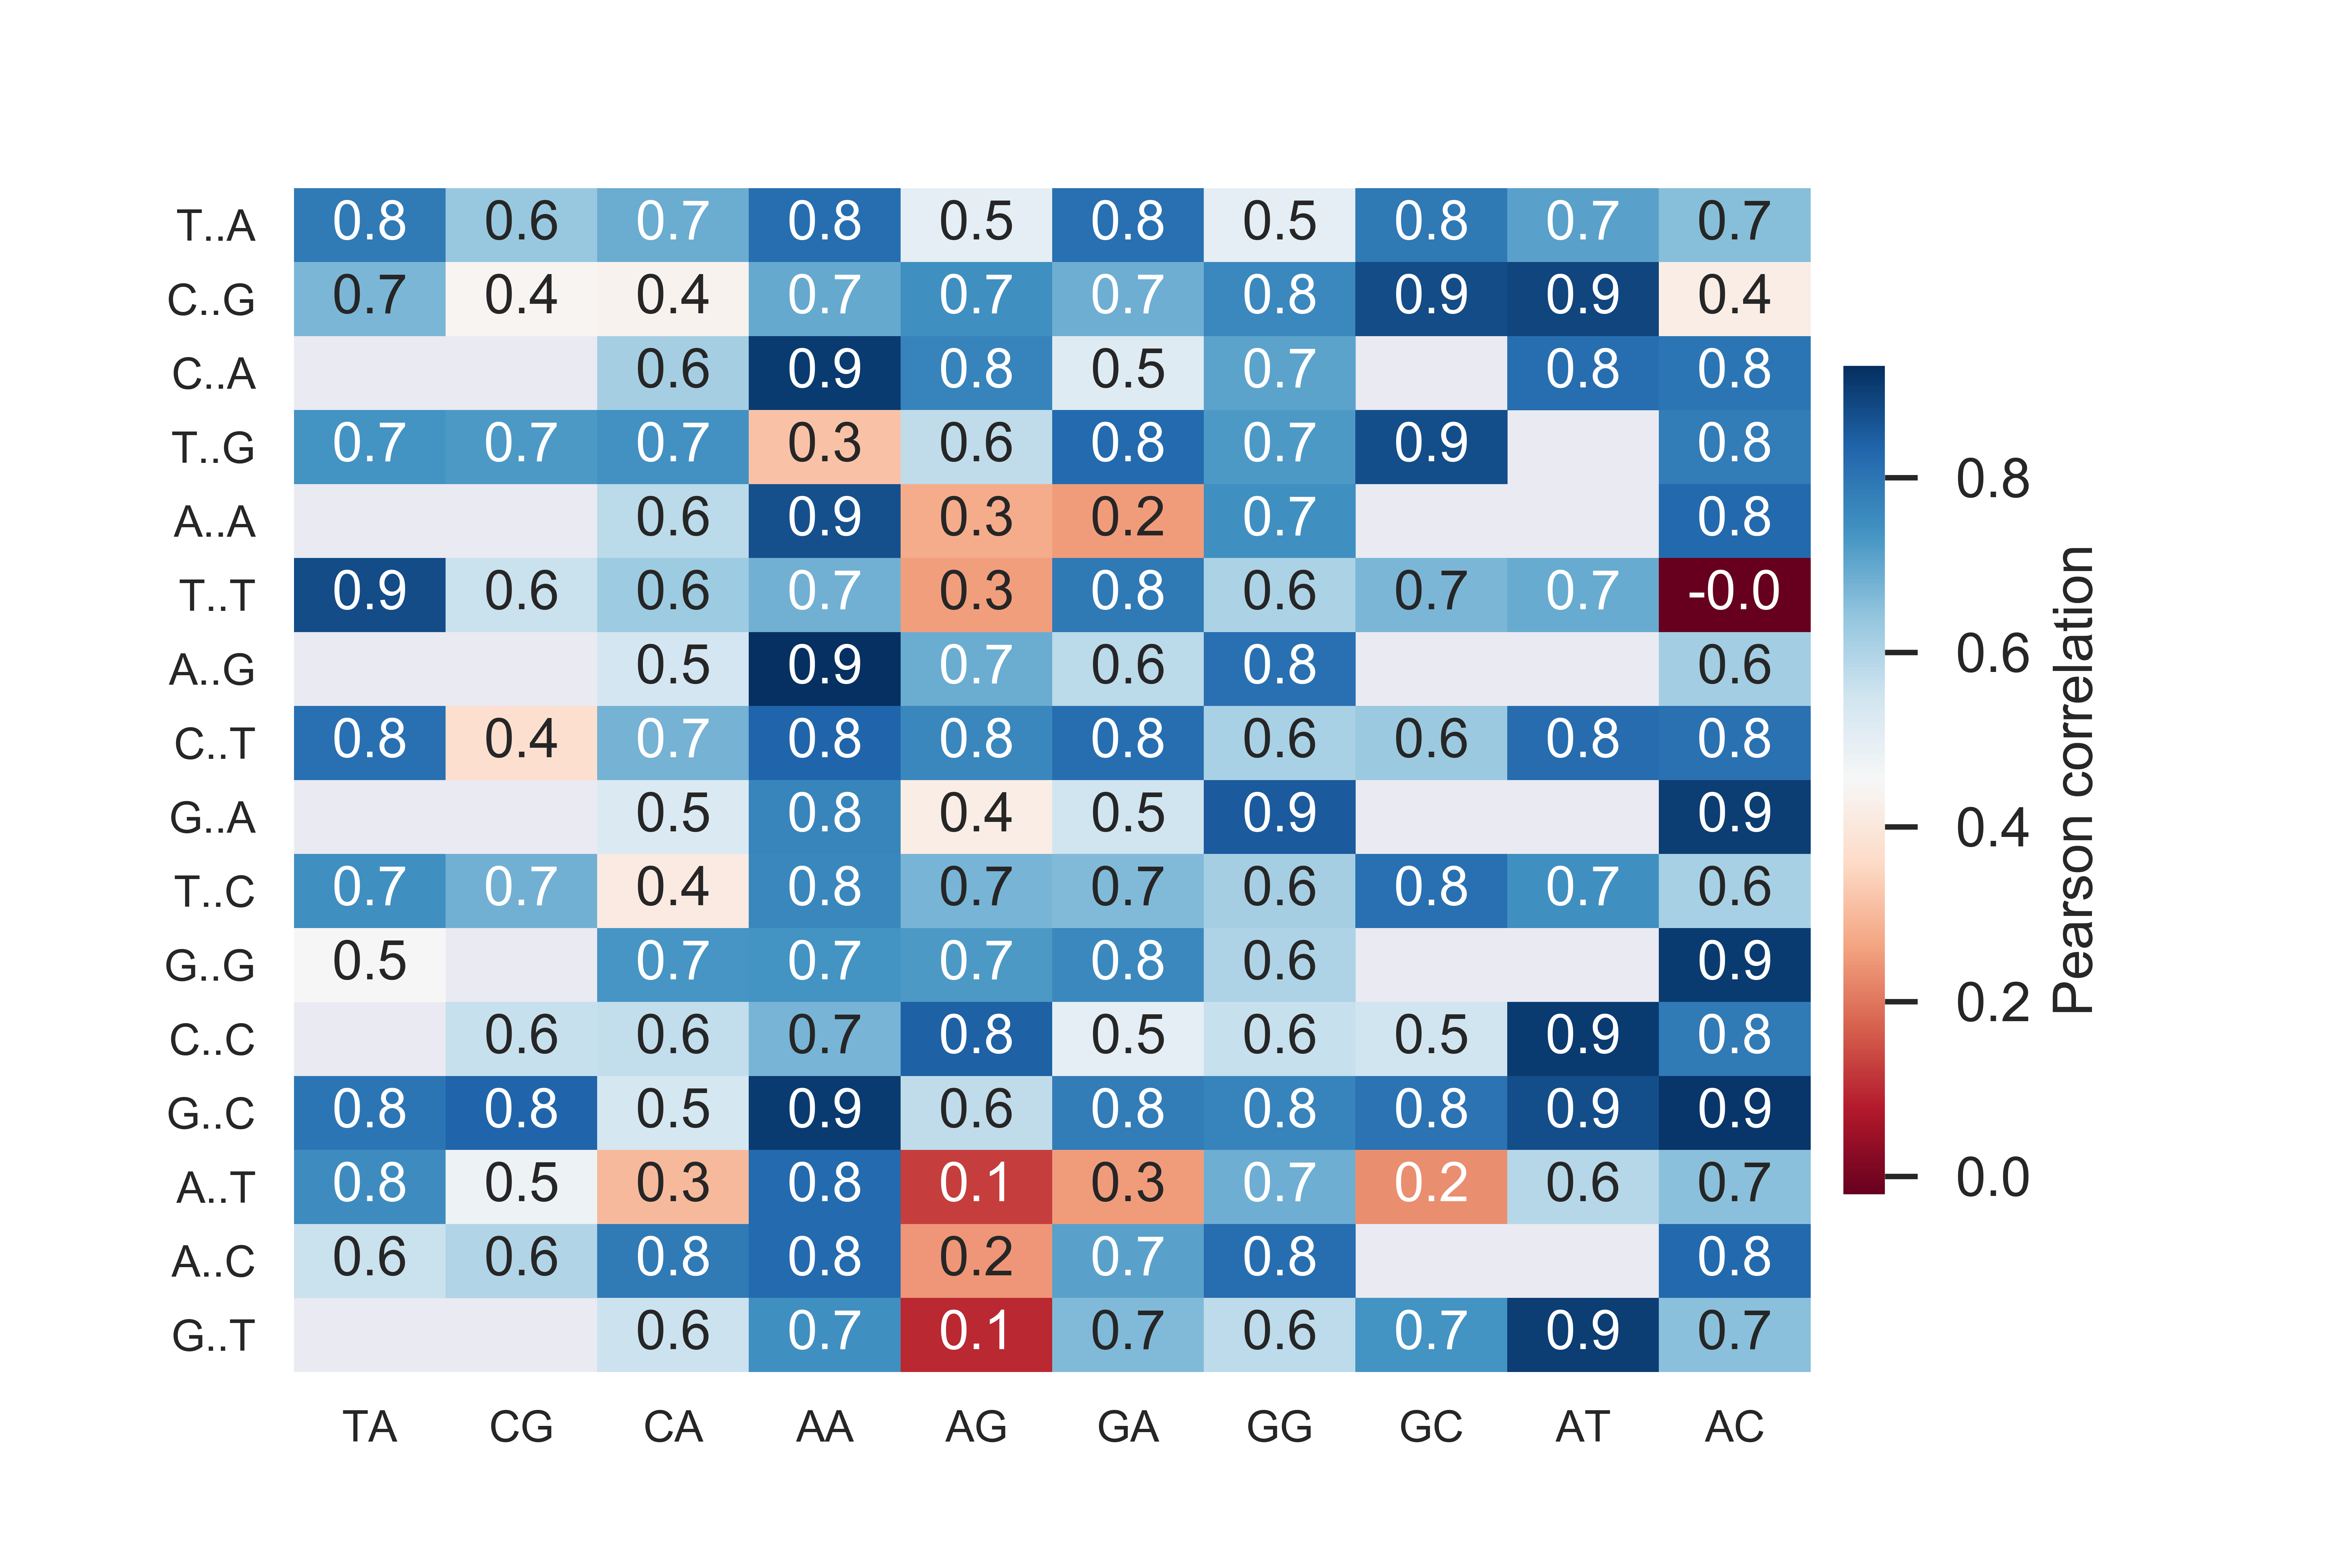
\includegraphics[scale=1]{./Xray_images/seq_var_heat_map_TX2.png}
% 	\caption{Difference in terms of linear correlation for dimer (in avg. flanking sequence ) with dimer in specific tetramer context in X-ray data set (case-\Rom{2}).  Abscissa is middle junction dimer-step and ordinate is tetramer context. The blank entries in the plot represent the dependent tetramer.
% 	}
% \label{SIfig:seq_var_heatmap_TX2}
% \end{center}
% \end{figure}


% \begin{figure}[H]
% 	\begin{center}
% 	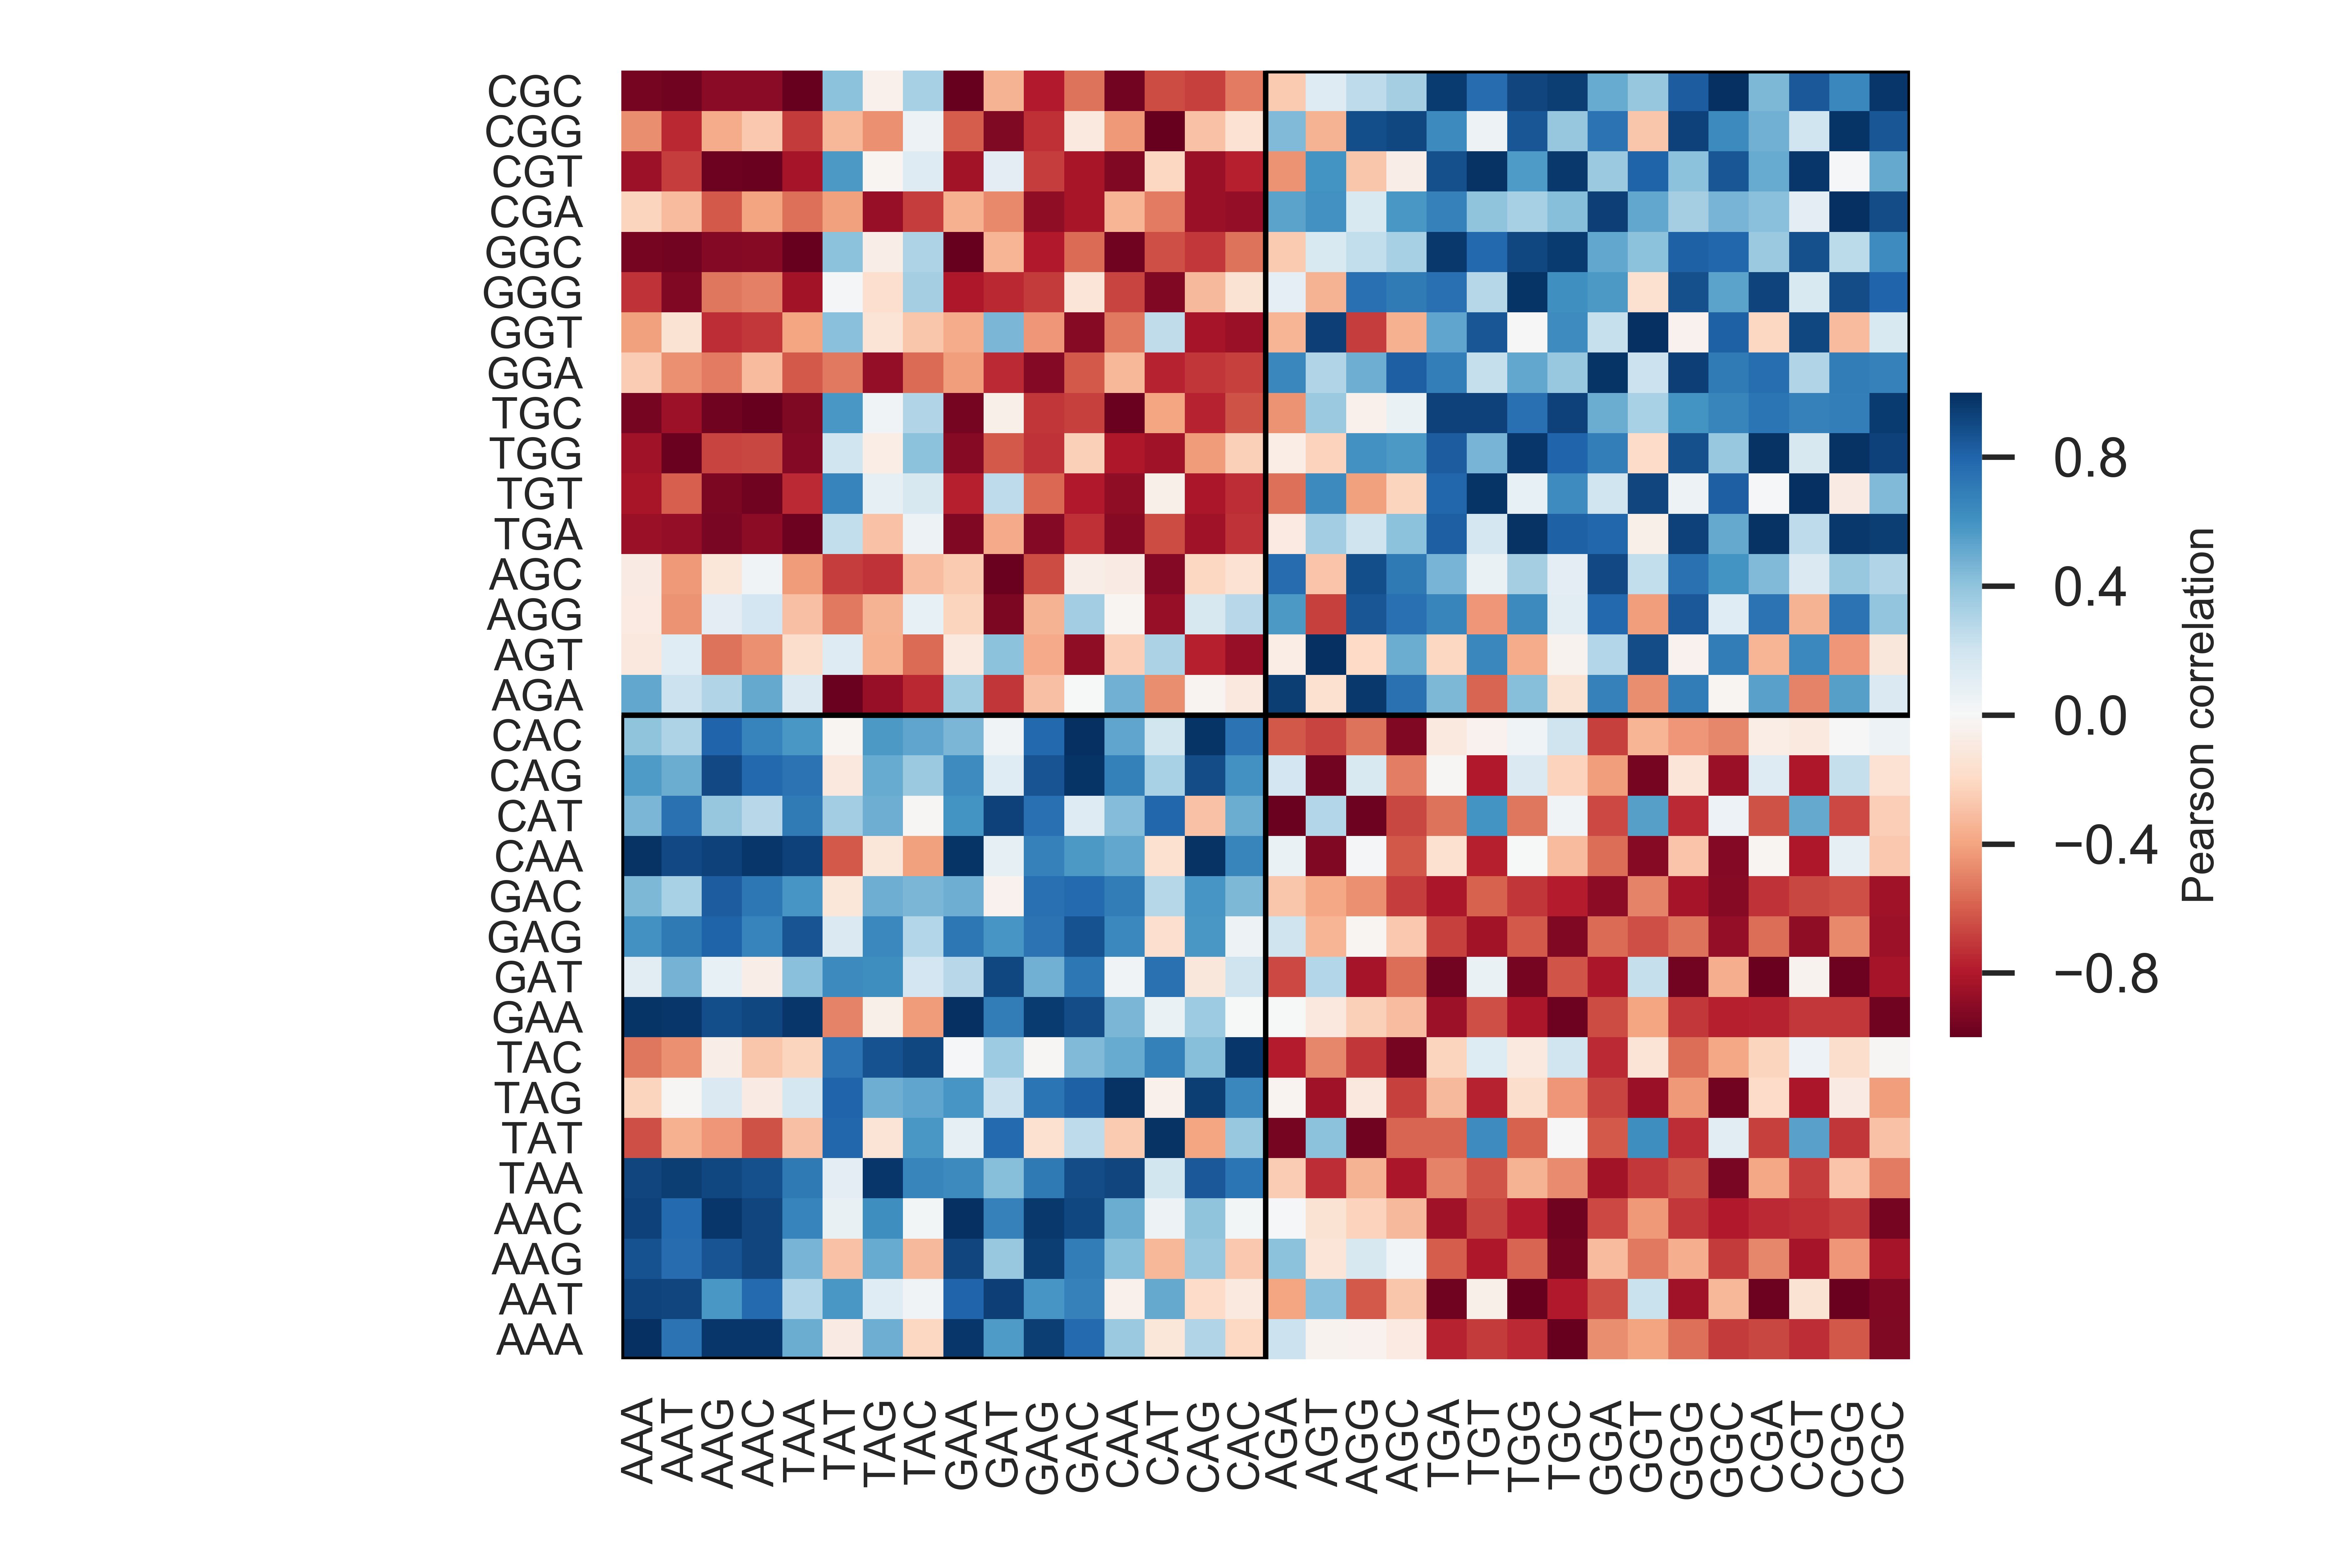
\includegraphics[scale=1]{./Xray_images/pearson_corr_mu_TX2_C1_CG_trimer_intra.png}
% 	\caption{cosine similarity (CoSim) between the groundstate of base-pairs (intra variables) in trimer context in X-ray (case-\Rom{2}) and cgNA$+$ data set on the diagonal entries. Whereas lower and upper off-diagonal is CoSim between different dimers in cgNA$+$ and X-ray data set, respectively. 
% 	}
% \label{SIfig:dim_comp_intra}
% \end{center}
% \end{figure}




% \begin{figure}
% 	\begin{center}
% 	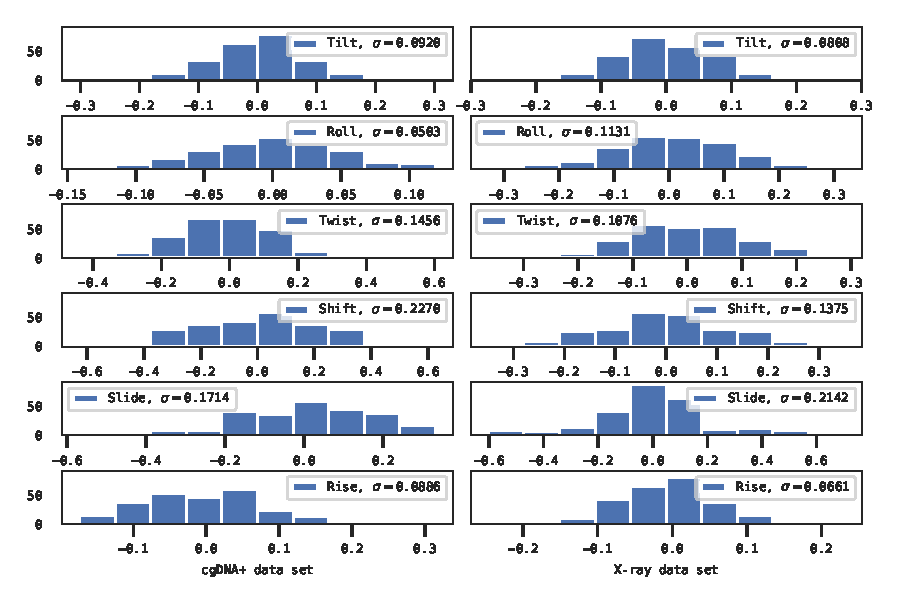
\includegraphics[scale=0.8]{./Xray_images/X3_logo_inter_mono-flank_bits_hist.pdf}
% 	\caption{Distribution for $\gamma_{\text{XUVY}}$ for inters as defined \cref{SIfig:logo_bits}}
% \label{SIfig:logo_hist}
% \end{center}
% \end{figure}

%%%%%%%%%%%%%%%%%%%%%%%%%%%%%%%%%%%%%%%%%%%%%%%%%%%%%%%%%%%%%%%%%%%%%%%%%%%%%%%%%
%%%%%%%%%%%%%%%%%%%%%%%%%%%%%%%%%%%%%%%%%%%%%%%%%%%%%%%%%%%%%%%%%%%%%%%%%%%%%%%%%%

%%%%%%%%%%%%%%%%%%%%%%%%%%%%%%%%%%%%%%%%%%%%%%%%%%%%%%%%%%%%%%%%%%%%%%%%%%%%%%%%%
%%%%%%%%%%%%%%%%%%%%%%%%%%%%%%%%%%%%%%%%%%%%%%%%%%%%%%%%%%%%%%%%%%%%%%%%%%%%%%%%%%

%%%%%%%%%%%%%%%%%%%%%%%%%%%%%%%%%%%%%%%%%%%%%%%%%%%%%%%%%%%%%%%%%%%%%%%%%%%%%%%%%
%%%%%%%%%%%%%%%%%%%%%%%%%%%%%%%%%%%%%%%%%%%%%%%%%%%%%%%%%%%%%%%%%%%%%%%%%%%%%%%%%%


% \section{Comparison of 3DNA and CURVES+} 






% \foreach \x in {1TGH,1JGR,1KX5,5WV7,6ON0}
% {   
% \begin{figure}
% 	\begin{center}
% 	\includegraphics[scale=0.8]{./Xray_images/\x_compare_3DNA_CURVE.pdf}
% 	\caption{Comparison of CURVES+ (in Solid) and 3DNA (in Dashed) for PDB id \x \; and the difference between the two is plotted in the next figure. Note to convert cgNA$+$ IC in degrees, we multiplied by the factor 36/pi.}
% \label{\x_compare_3DNA_CURVE}
% \end{center}
% \end{figure}
% \begin{figure}
% \begin{center}
% \includegraphics[scale=0.8]{./Xray_images/\x_diff_3DNA_CURVE.pdf}
% \caption{difference of CURVES+ and 3DNA for PDB id \x 
% 	}
% \label{\x_compare_3DNA_CURVE}
% \end{center}
% \end{figure}
% }





%%%%%%%%%%%%%%%%%%%%%%%%%%%%%%%%%%%%%%%%%%%%%%%%%%%%%%%%%%%%%%%%%%%%%%%%%%%%%%%%%
%%%%%%%%%%%%%%%%%%%%%%%%%%%%%%%%%%%%%%%%%%%%%%%%%%%%%%%%%%%%%%%%%%%%%%%%%%%%%%%%%%

%%%%%%%%%%%%%%%%%%%%%%%%%%%%%%%%%%%%%%%%%%%%%%%%%%%%%%%%%%%%%%%%%%%%%%%%%%%%%%%%%
%%%%%%%%%%%%%%%%%%%%%%%%%%%%%%%%%%%%%%%%%%%%%%%%%%%%%%%%%%%%%%%%%%%%%%%%%%%%%%%%%%

%%%%%%%%%%%%%%%%%%%%%%%%%%%%%%%%%%%%%%%%%%%%%%%%%%%%%%%%%%%%%%%%%%%%%%%%%%%%%%%%%
%%%%%%%%%%%%%%%%%%%%%%%%%%%%%%%%%%%%%%%%%%%%%%%%%%%%%%%%%%%%%%%%%%%%%%%%%%%%%%%%%%

\section{Comparison of two X-ray data sets with different resolutions and results for case-\rom{2}} 
\begin{figure}
	\begin{center}
	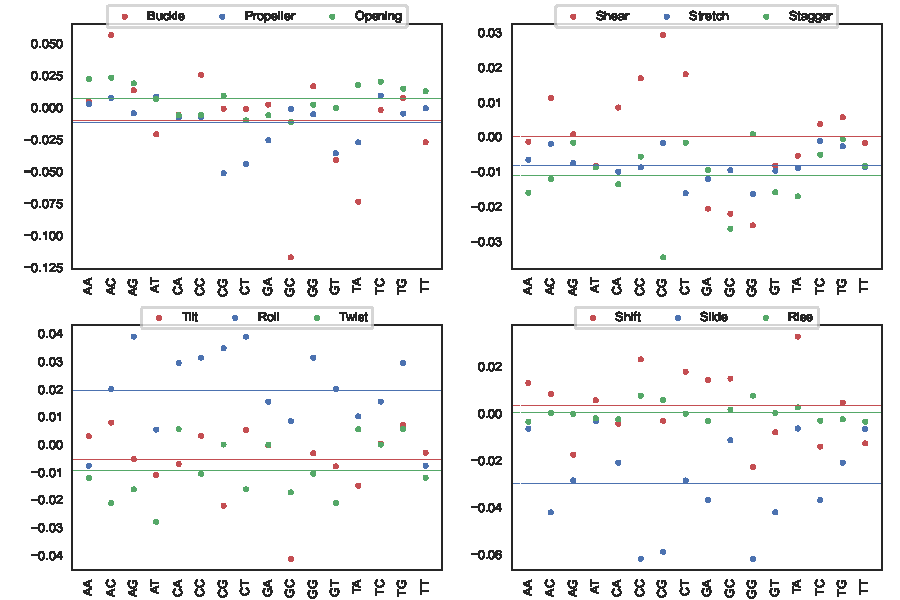
\includegraphics[scale=0.8]{./Xray_images/muDX2-muDX3_diff_compare_res.pdf}
	\caption{Plot comparing the average shape of dimer in two X-ray datasets as defined in case-\Rom{1} and case-\Rom{2} where case-\Rom{1} has no resolution cut-off and case-\Rom{2} has data only resolution better that 3 \AA \; in \cref{Database}. In this figure, we have plotted the difference in average shape of dimers in average context as the scatter plot and \textbf{dashed} line is the average difference between two data sets for a given internal coordinate.}
\label{SIfig:dimer_diff_res_compare}
\end{center}
\end{figure}

\begin{figure}
	\begin{center}
	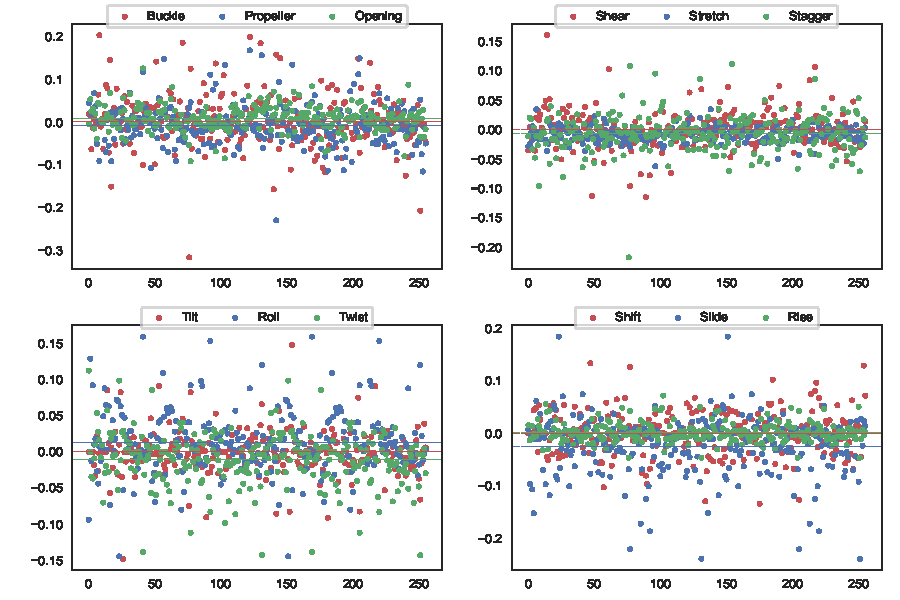
\includegraphics[scale=0.8]{./Xray_images/muTX2-muTX3_diff_compare_res.pdf}
	\caption{Plot comparing the average shape of dimer in two X-ray data sets as defined in case-\Rom{1} and case-\Rom{2} where case-\Rom{1} has no resolution cut-off and case-\Rom{2} has data only resolution better that 3 \AA \; in \cref{Database}. In this figure, we have plotted the difference in average shape of tetramers as the scatter plot and dashed line is the average difference between two data sets for a given internal coordinate.}
\label{SIfig:tet_diff_res_compare}
\end{center}
\end{figure}

%%%%%%%%%%%%%%%%%%%%%%%%%%%%%%%%%%%%%%%%%%%%%%%%%%%%%%%%%%%%%%%%%%%%%%%%%%%%%%%%%
%%%%%%%%%%%%%%%%%%%%%%%%%%%%%%%%%%%%%%%%%%%%%%%%%%%%%%%%%%%%%%%%%%%%%%%%%%%%%%%%%%


\begin{figure}[H]
	\begin{center}
	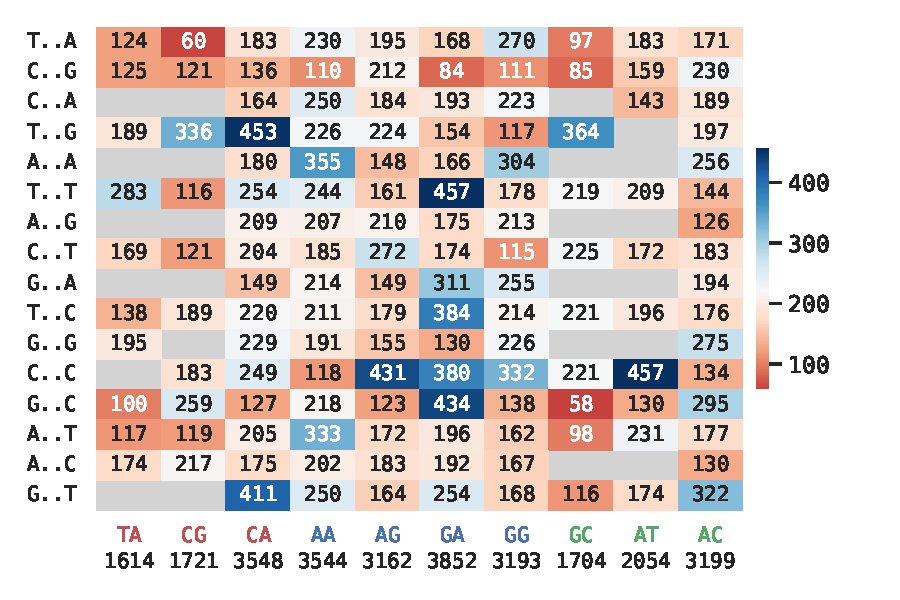
\includegraphics[scale=0.75]{./Xray_images/freq_heat_map_tt2_3S_C1_cg_unsym.pdf}
	\caption{Number of appearances of 136 tetrameters in X-ray  data set (case-\Rom{2}). Abscissa is middle junction dimer-step and ordinate is tetramer context. Note that the palindromic steps are only read from reading strand.}
\label{SIfig:freq}
\end{center}
\end{figure}

\begin{figure}[H]
	\begin{center}
	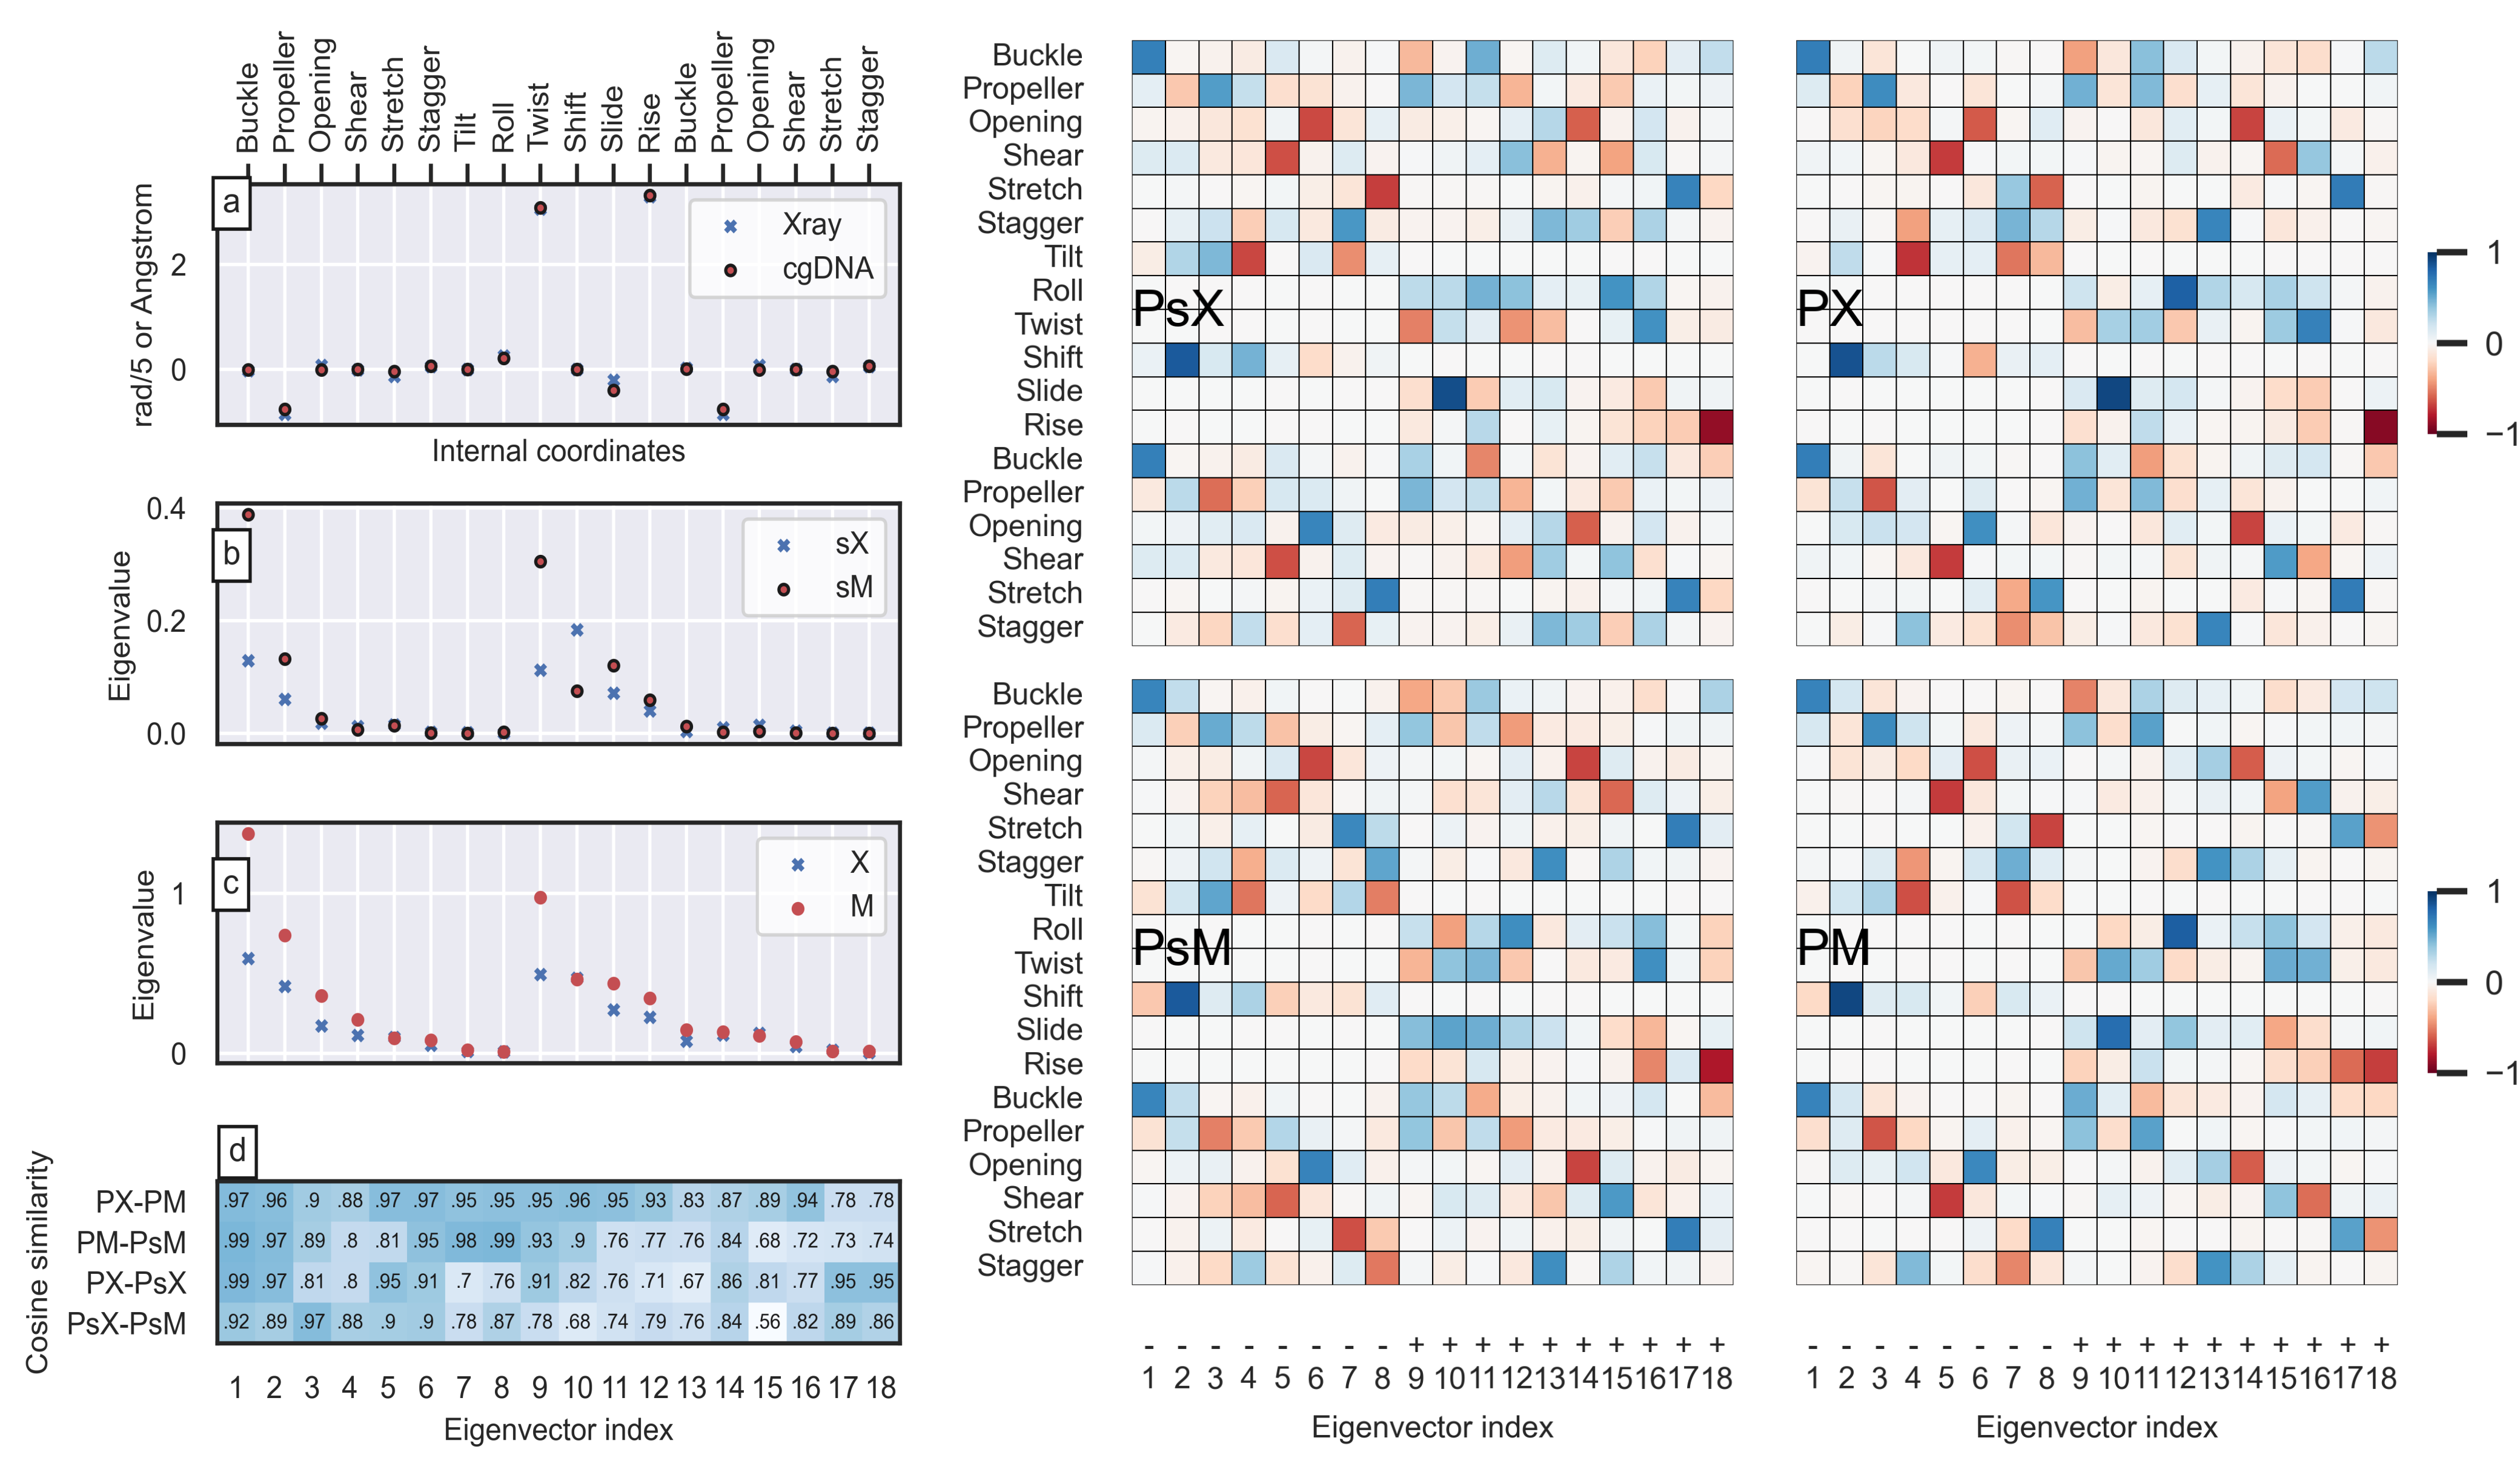
\includegraphics[scale=0.9]{./Xray_images/X2_PP.png}
	\caption{a) Plot comparing sequence-independent groundstate (average shape) of dimer coordinates in X-ray (case-\Rom{2}) and cgNA$+$ model data set. On right, $P_sX$ and $P_sM$ are the associated eigenvector matrices for the shape covariance matrix (denoted by subscript s) describing the directions of variation in groundstate over sequence space for X-ray (denoted by superscript X) and cgNA$+$ model (denoted by superscript M) data sets, respectively and $D_sX$ and $D_sM$ are corresponding eigenvalues in b). While $PX$ and $PM$ are the eigenvectors of average configuration covariance 
	describing the direction of deformation of DNA in configuration space and $DX$ and $DM$ are corresponding eigenvalues in c). In d), there is cosine similarity index for corresponding eigenvectors in ($CX,CM$), ($C_sM,CM$), ($C_sX,CX$), and ($C_sX,C_sM$).  
	}
\label{SIfig:PMPX}
\end{center}
\end{figure}

\begin{figure}[H]
	\begin{center}
	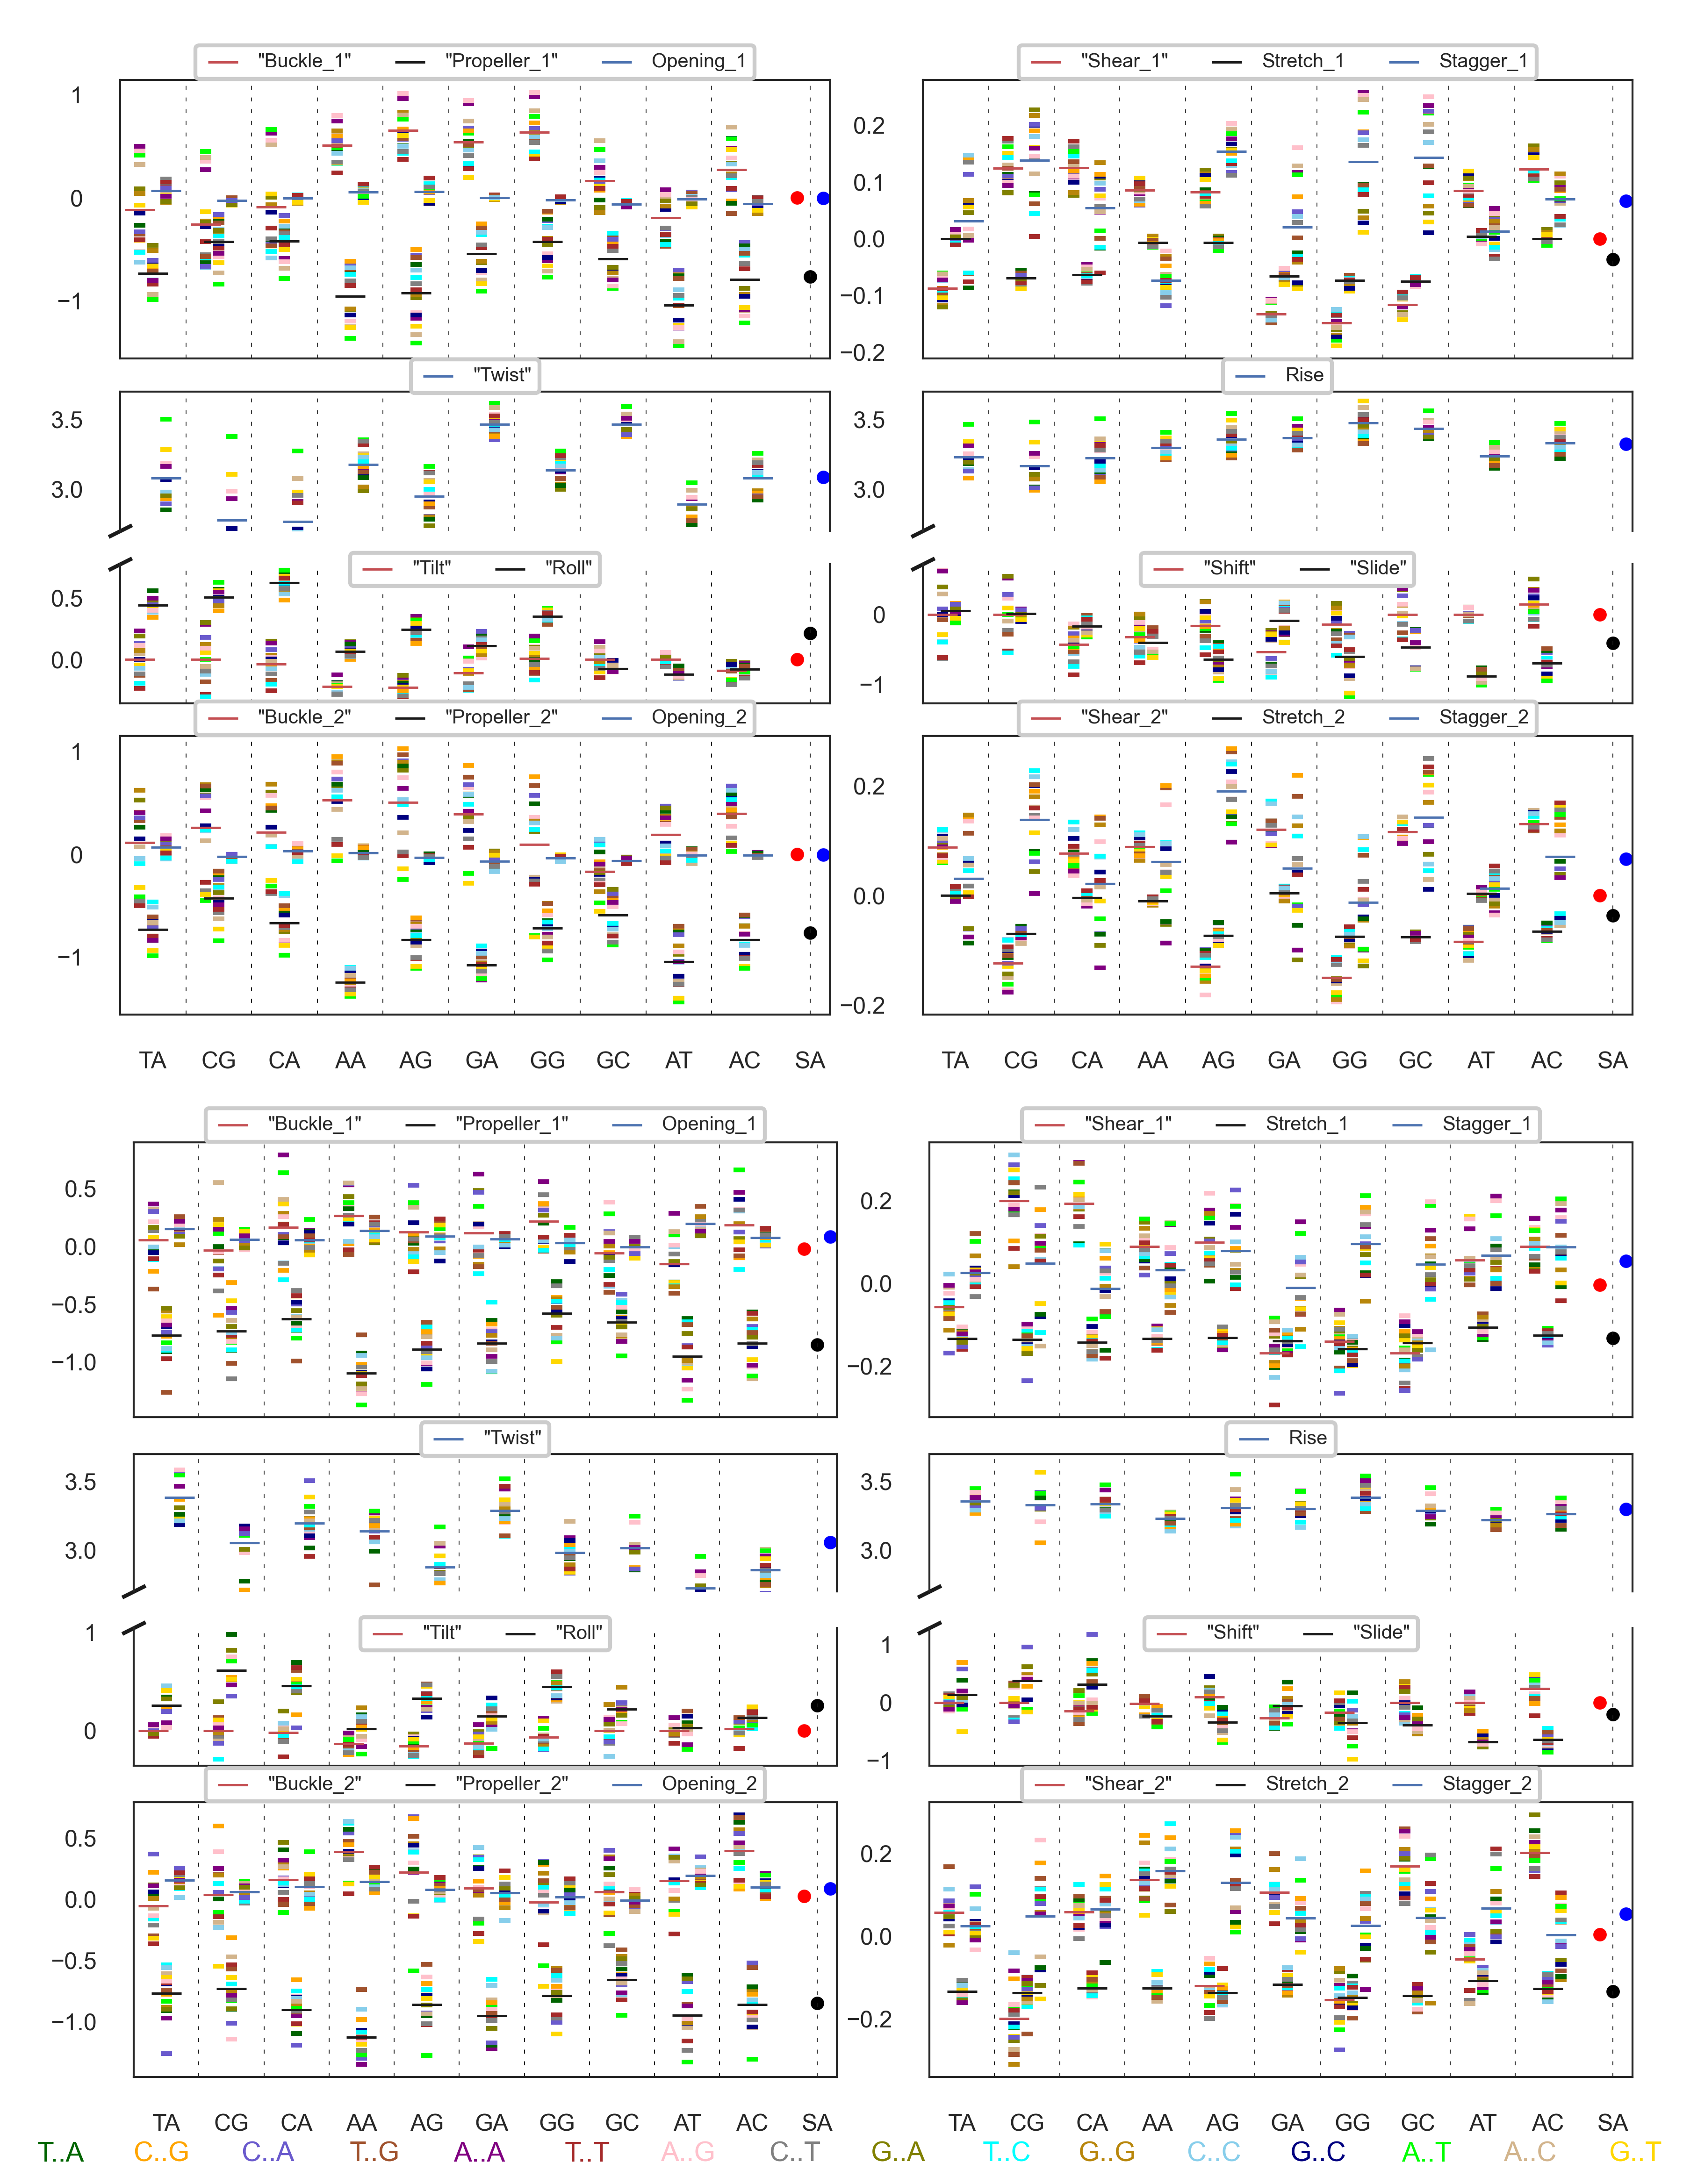
\includegraphics[scale=1]{./Xray_images/seq_var_combine_X2.png}
	\caption{Plot of Intras and Inter for X-ray, case-\Rom{2} (bottom) and cgNA$+$ model (top) data set in which large dash lines depict ICs of a dimer (in average context) while the other smaller dash lines are the ICs for that dimer in a specific tetramer context. For a better and more concise visual representation, the three ICs are slightly shifted on the X-axis in each subplot. Also, various flanking contexts are plotted in different colors, as described at the bottom of the plot. SA is sequence-average groundstate.
	}
\label{SIfig:seq_imp2}
\end{center}
\end{figure}

\begin{figure}
	\begin{center}
	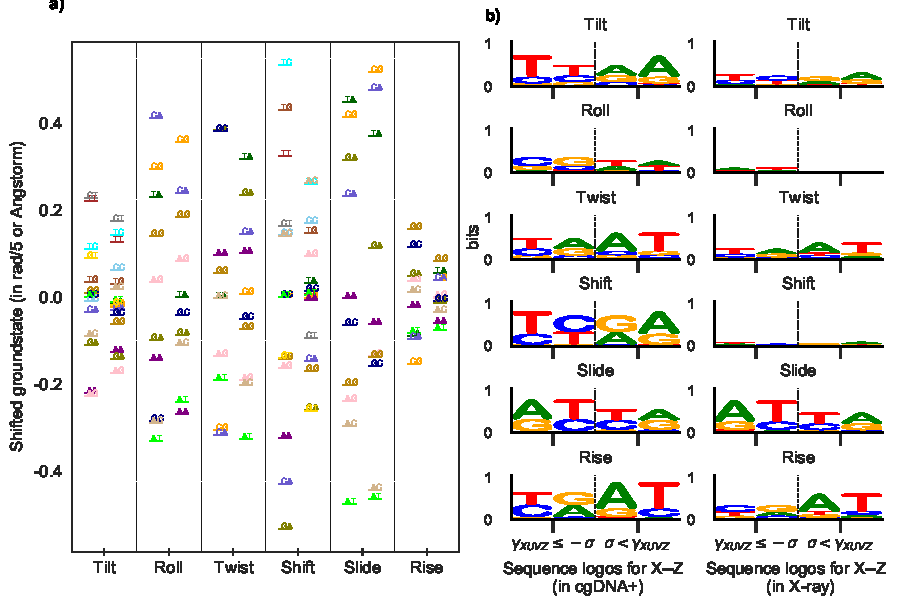
\includegraphics[scale=1]{./Xray_images/X2_logo_inter_mono-flank_bits.pdf}
	\caption{
a) Inter ICs (shifted with respect to sequence-average groundstate) are plotted for dimers in average flanking context to identify which dimers assume distant values from sequence-average groundstate for a given variable and whether that signal is consistent in the two data sets. The left column is for the cgNA$+$ model data set for each IC, and the right column is for the X-ray data set. b)
Sequence logo plot to statistically quantify
the role of tetramer context on the ground-state (in inter variables) of a given dimer.
For each internal coordinate (IC), we have defined $\gamma_{\text{XUVZ}}= \text{IC}_{\text{XUVZ}} - \text{IC}_{\text{X}_{\text{avg}}\text{UV}\text{Z}_{\text{avg}}}$ as the difference of the internal coordinate of a dimer (UV) in tetramer context (X\,-\,-\,Z) with the same dimer in average context, where X, U, V, Z $\in$ [A, T, C, G]. 
Then, for each internal coordinate, we have defined positive and negative outliers as, $ \gamma_{\text{XUVZ}} < -\sigma$
and $ \gamma_{\text{XUVZ}} > +\sigma$, 
where $\sigma$ is standard deviation of $\gamma_{\text{XUVZ}}$.
In the sequence-logo plot, we have plotted the information content in the tetramer flanking context (X\,-\,-\,Z) for which $\gamma_{\text{XUVZ}}$ are negative or positive outliers.
}
\label{SIfig:logo_bits}
\end{center}
\end{figure}


\begin{figure}[H]
	\begin{center}
	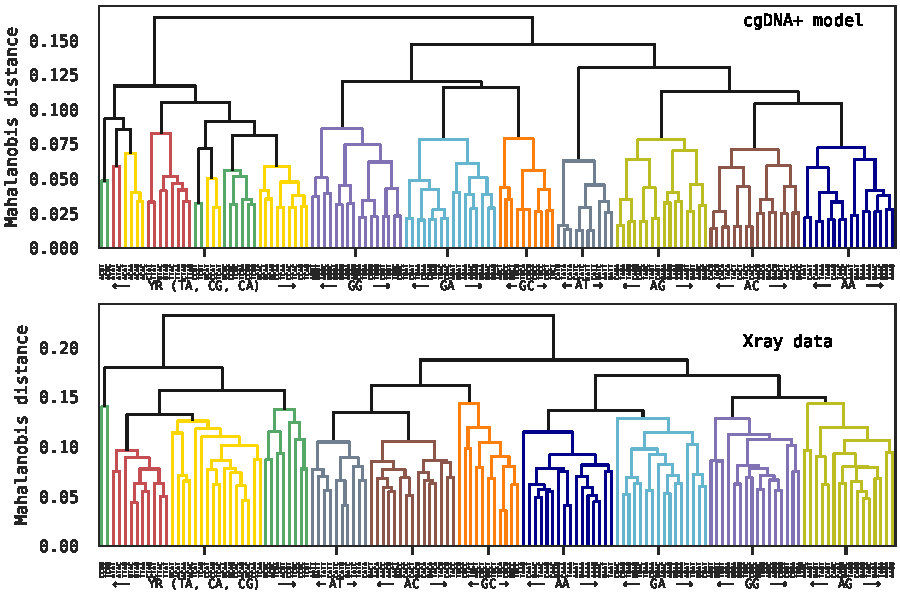
\includegraphics[scale=1]{./Xray_images/Dendrogram_cgxray_X2.pdf}
	\caption{Dendrograms using hierarchical clustering on independent tetramers using Mahalanobis distance (taking inverse of sequence-dependent configuration covariance as the weight matrix) and average linkage algorithm \cref{ss:cluster}.  %Note that the outliers in the dendrogram for X-ray data set have higher number of appearances in the X-ray crystal database. Namely, TCGG (387), GCAT (495), CGAC (428), and TGCG (411). 
	}
\label{SIfig:cluster}
\end{center}
\end{figure}

\begin{figure}[H]
	\begin{center}
	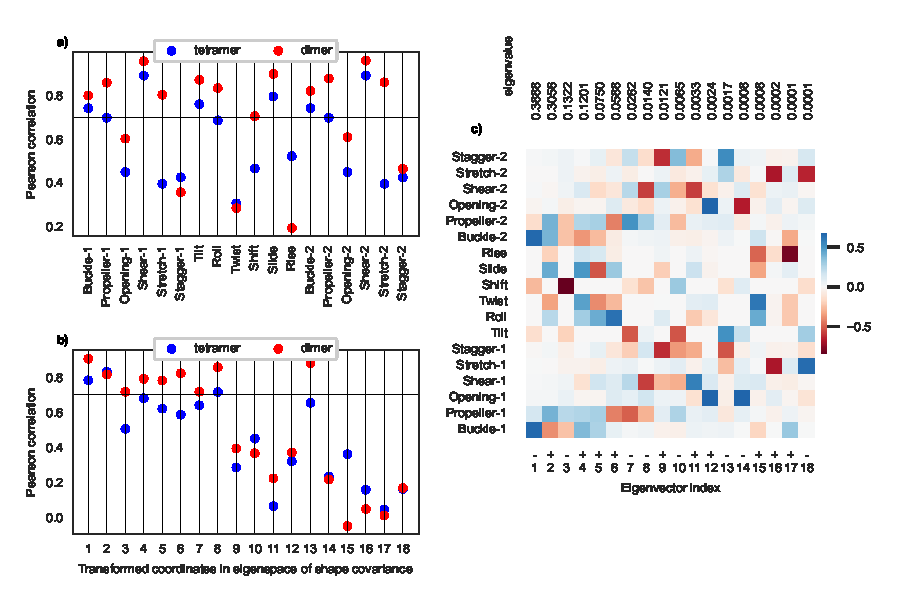
\includegraphics[scale=0.9]{./Xray_images/X2_CG_256_PC_one_one.pdf}
	\caption{Pearson correlation between X-ray (case-\Rom{2}) and cgNA$+$ data set in a) standard CURVES$+$ coordinates and b) transformed coordinates in eigenspace of cgNA$+$ shape covariance and corresponding eigenvectors shown in c) with $+/-$ parity as defined in \cref{ss:parity}.
	}
\label{SIfig:PC_one_one}
\end{center}
\end{figure}

\begin{figure}[H]
	\begin{center}
	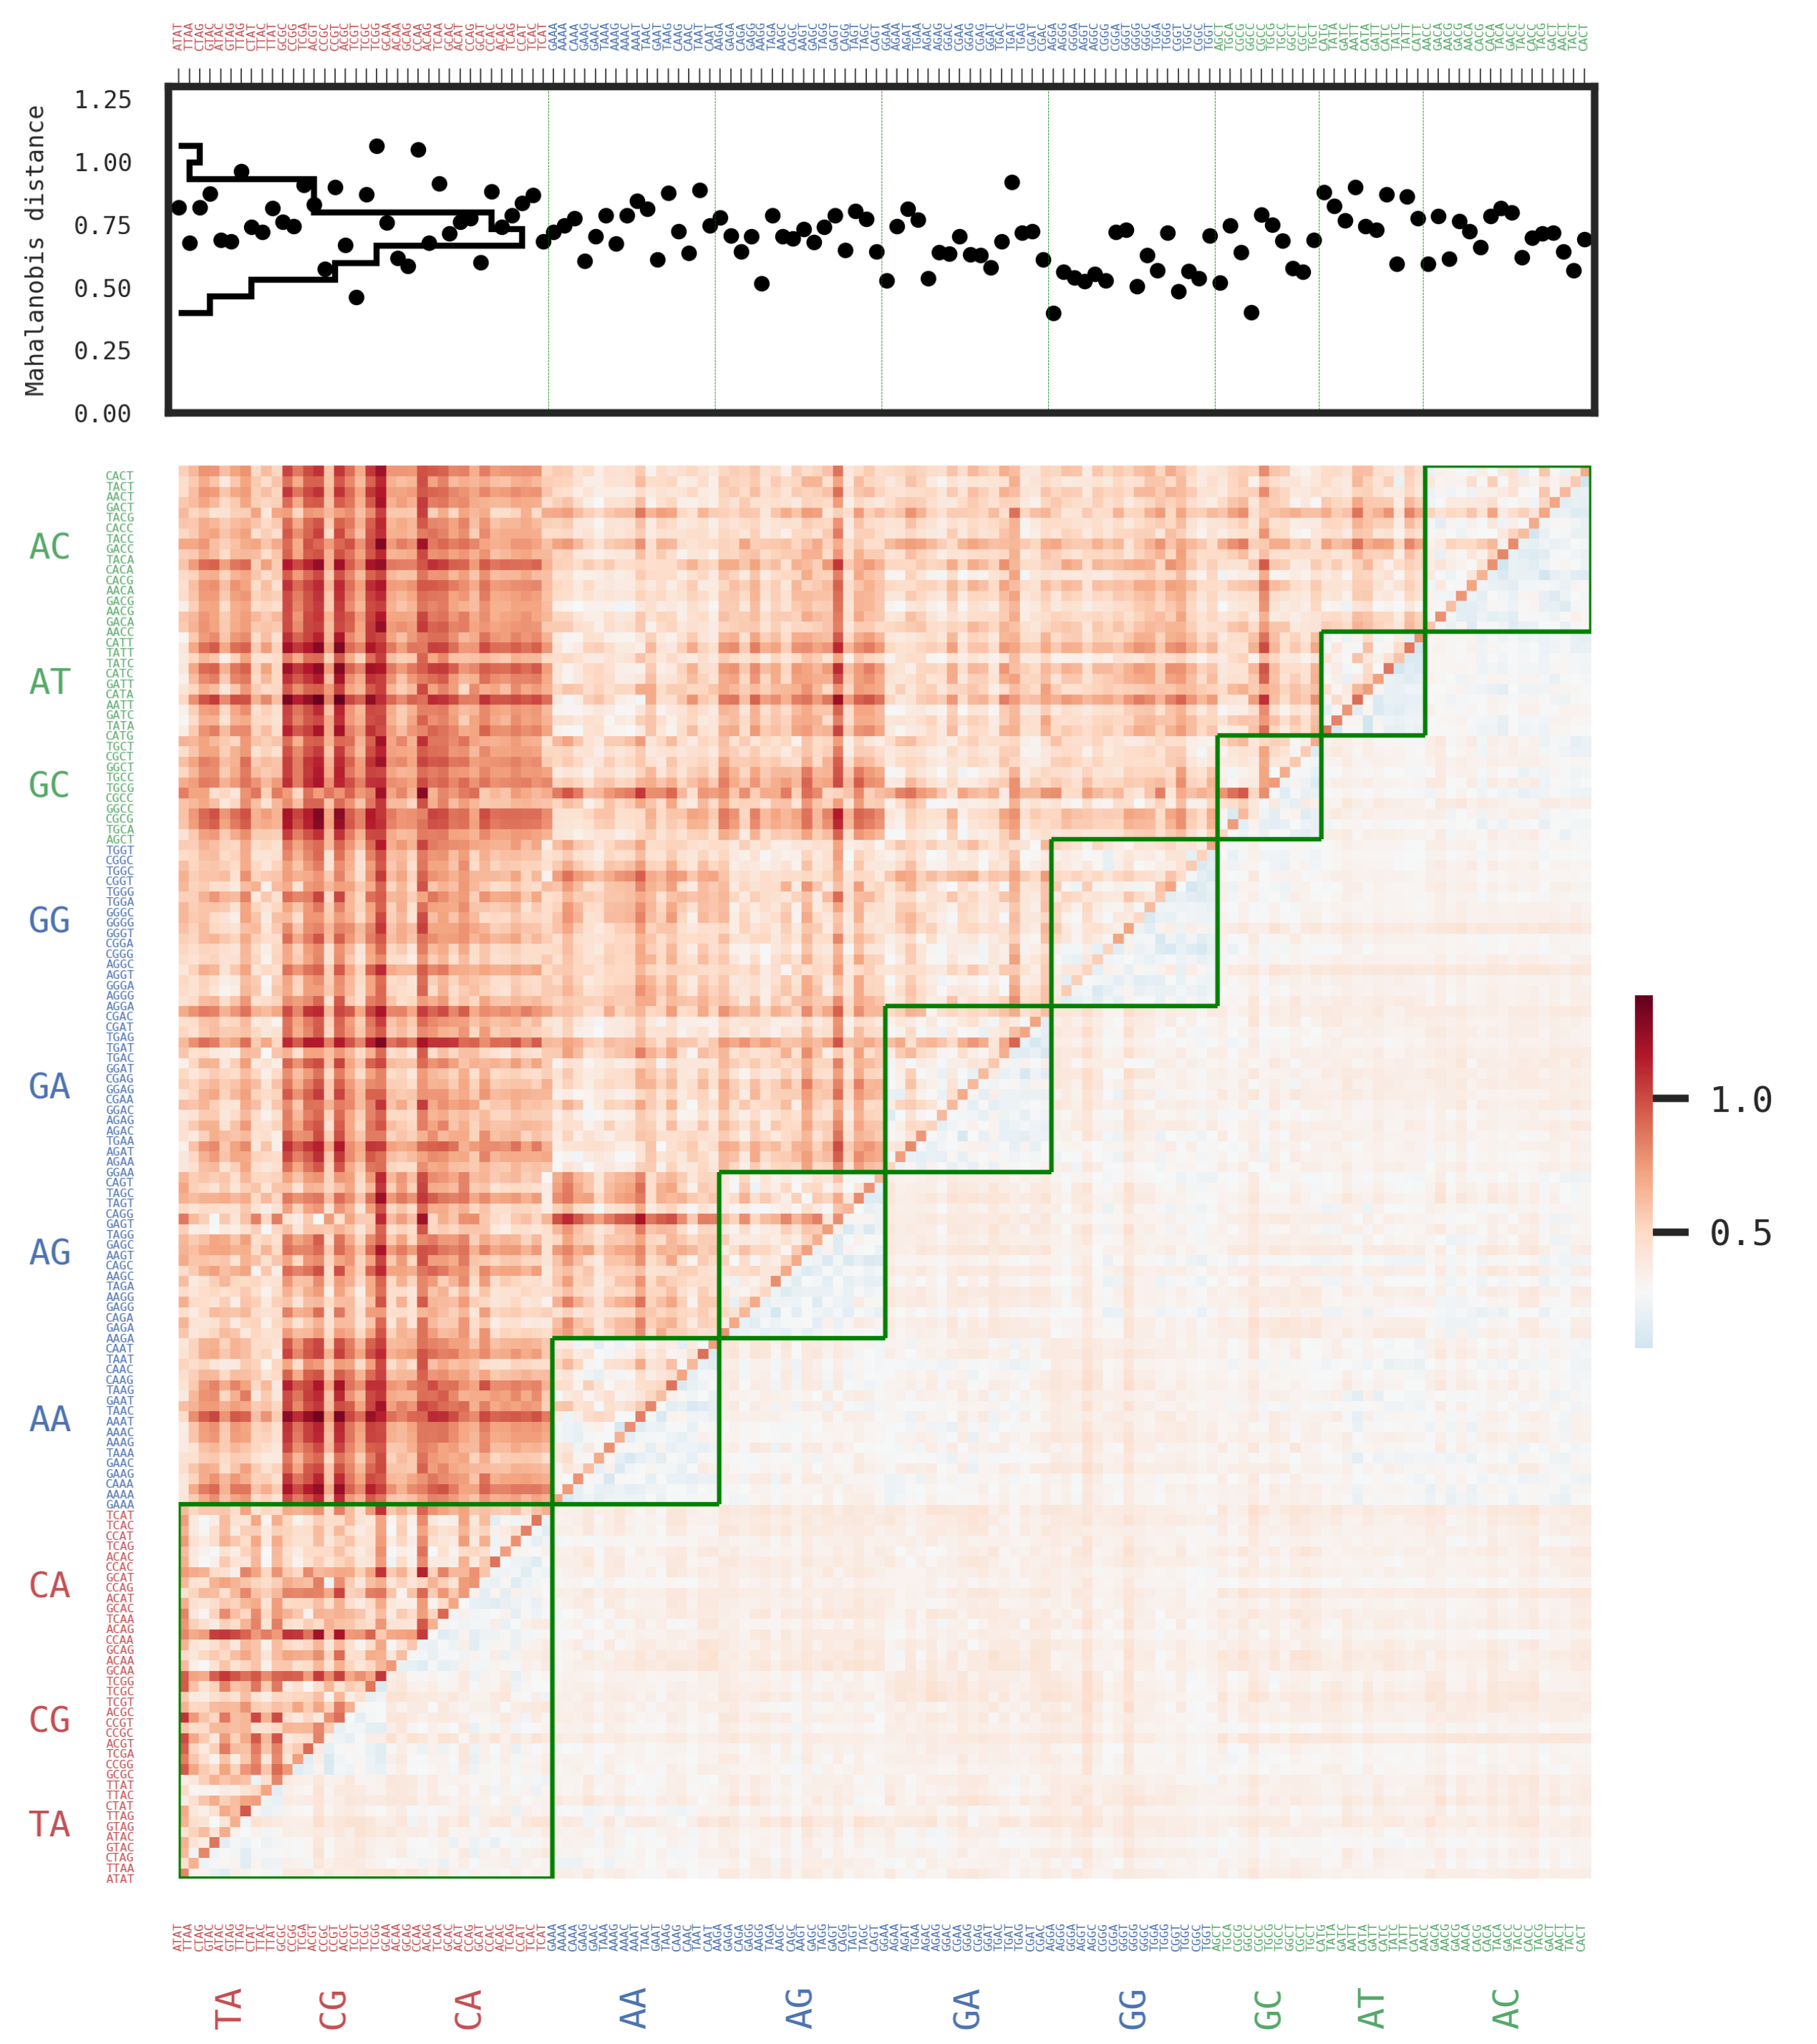
\includegraphics[scale=1.45]{./Xray_images/X2_heat_mahal_pca_18_comb.png}
	\caption{
	In the heat map (bottom), the diagonal entries are Mahalanobis distance between the groundstate of dimers (in 136 independent tetramer contexts) in X-ray and cgNA$+$ model data set. Whereas lower and upper off-diagonal entries are Mahalanobis distance between different dimers (in specific tetramer context) within cgNA$+$ model and X-ray data set, respectively. The diagonal entries of heat-map are again plotted in scatter plot (top) along with the histogram in the same plot.
	Note that the Mahalanobis distance (defined in \cref{c2:s5sb3}) is computed in the 18 CURVES$+$ coordinates and using cgNA$+$ shape covariance matrix as weight matrix. 
    }
\label{SIfig:Mahal_18}
\end{center}
\end{figure}

\begin{figure}[H]
	\begin{center}
	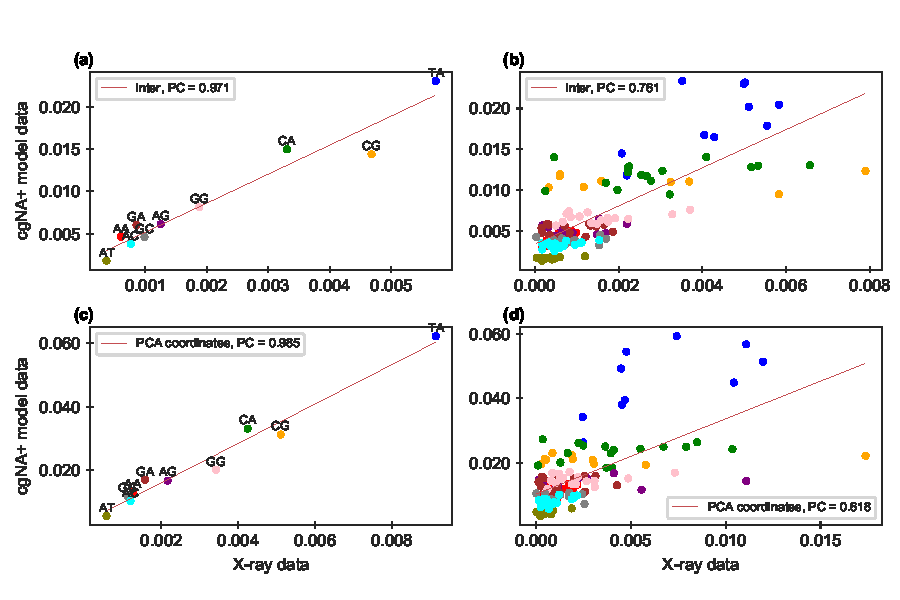
\includegraphics[scale=0.9]{./Xray_images/vol_R2_DX2_3S_C1_cg.pdf}
	\caption{Comparison of configurational volume
	for cgNA$+$ model covariance vs X-ray data set (case-\Rom{2}) covariance a) in inter coordinates for independent dimer steps in average context, b) in inter coordinates for dimers in independent tetramer contexts, c) in PCA coordinates (in  eight principal modes of cgNA$+$ model shape covariance $\in \R^{18}$) for independent dimer steps in average context, d) in PCA coordinates (in  eight principal modes of cgNA$+$ model shape covariance $\in \R^{18}$) for dimers in independent tetramer contexts.}
% Note that the unit of S can be assumed \AA$^{N/2}\cdot(rad/5)^{N/2}$.
\label{SIfig:TX3stiff}
\end{center}
\end{figure}

\begin{figure}[H]
	\begin{center}
	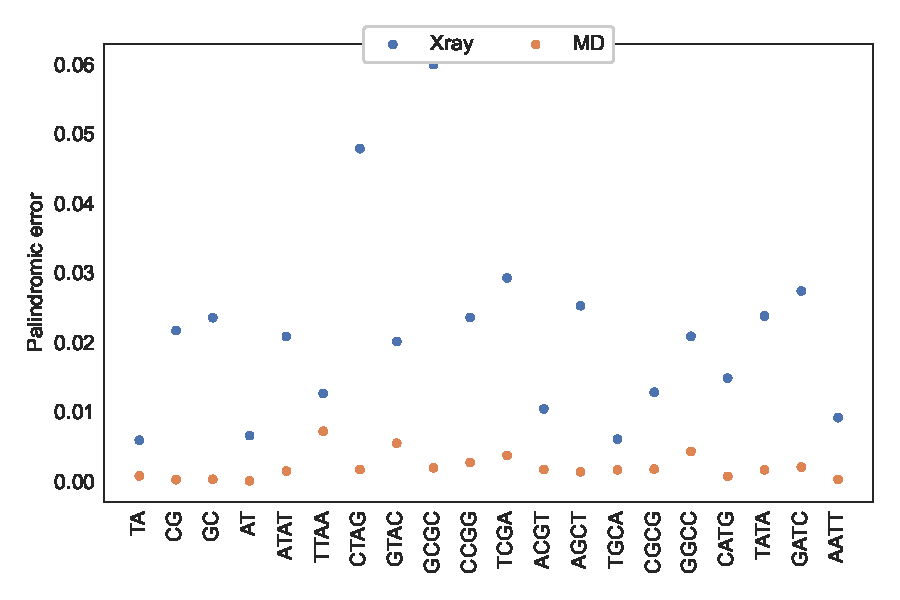
\includegraphics[scale=0.8]{./Xray_images/palin_err_tt2_3S_C1_cg_unsym.pdf}
	\caption{
    Palindromic error (as defined in \cref{c2:s5sb1}) per degree of freedom in the groundstate of palindromic dimer in tetramer flanking context and in average flanking context for X-ray data set (Case-\Rom{2}) and MD simulations (used to train cgNA$+$ model). 
%    As described in \cref{ss:parity}, groundstate ($\mu$) for palindromic dimer should be invariant of the reading strand which allows us to define the palindromic error as $|\mu-E\mu|$ to quantify the convergence of groundstate where $E$ is reading strand transformation matrix defined in \cref{SIeq:Ematint}. Even though the palindromic error is a norm of a vector with mixed rotational and translational entries, the length scale of palindromic error can be treated in \AA \; or rad/5 units.
	}
\label{SIfig:palin_error_X2}
\end{center}
\end{figure}


% \begin{table}[H]
% \begin{tabular}{ccc|c|ccc|c|c}
% seq & tilt &roll &  twist  &  tilt &roll & twist  &  total rot &  bp per turn \\
%  &   & \textbf{3DNA coords} &  && \textbf{cgNA$+$ coords}  &  &  & using tot rot \\
% \hline
% &&&& MD data &&&&\\
% \hline
% TA & -0.0 & 4.83 & 34.22 & 0.0 & 5.05 & 35.28 & 34.55 &  \\
% CG & 0.0 & 5.58 & 31.03 & 0.0 & 5.79 & 31.82 & 31.52 &  \\
% CA & -0.39 & 6.86 & 30.92 & -0.4 & 7.13 & 31.7 & 31.66 &  \\
% AA & -2.4 & 0.74 & 35.25 & -2.51 & 0.77 & 36.41 & 35.34 & 10.19 \\
% AG & -2.49 & 2.68 & 32.85 & -2.6 & 2.8 & 33.78 & 33.05 &  \\
% GA & -1.19 & 1.22 & 38.21 & -1.26 & 1.29 & 39.69 & 38.25 &  \\
% GG & 0.1 & 3.82 & 34.82 & 0.1 & 4.01 & 35.94 & 35.03 & 10.28 \\
% GC & -0.0 & -0.79 & 38.21 & 0.0 & -0.84 & 39.69 & 38.21 &  \\
% AT & 0.0 & -1.32 & 32.25 & 0.0 & -1.38 & 33.13 & 32.27 &  \\
% AC & -0.99 & -0.86 & 34.24 & -1.04 & -0.9 & 35.3 & 34.26 &  \\
% Avg & 0.0 & 2.32 & 34.28 & -0.0 & 2.43 & 35.35 & 34.36 & 10.48 \\
% \hline
% &&&& X-ray data &&&&\\
% \hline
% TA & -0.0 & 2.68 & 37.22 & -0.0 & 2.83 & 38.59 & 37.32 &  \\
% CG & -0.0 & 6.33 & 34.06 & -0.0 & 6.63 & 35.1 & 34.62 &  \\
% CA & -0.25 & 5.09 & 35.44 & -0.27 & 5.35 & 36.62 & 35.8 &  \\
% AA & -1.41 & -0.03 & 35.18 & -1.48 & -0.03 & 36.33 & 35.21 & 10.23 \\
% AG & -1.85 & 3.31 & 32.16 & -1.93 & 3.44 & 33.03 & 32.38 &  \\
% GA & -1.54 & 1.7 & 36.42 & -1.62 & 1.79 & 37.7 & 36.49 &  \\
% GG & -0.64 & 4.5 & 33.32 & -0.66 & 4.7 & 34.3 & 33.62 & 10.71 \\
% GC & 0.0 & 2.29 & 33.64 & 0.0 & 2.39 & 34.65 & 33.72 &  \\
% AT & -0.0 & 0.12 & 30.84 & -0.0 & 0.13 & 31.61 & 30.84 &  \\
% AC & 0.1 & 1.41 & 32.09 & 0.11 & 1.47 & 32.96 & 32.12 &  \\
% Avg & -0.0 & 2.71 & 34.07 & -0.0 & 2.84 & 35.11 & 34.18 & 10.53 \\
% \end{tabular}
% \caption{
% From the relative rotation matrix between the adjacent base-pairs, we obtained cgNA$+$ and 3DNA coordinates (first two columns). It highlights the difference between two kinds of coordinates. 
% Total rotation is the $2 arctan^{-1} (|u|/10)$ where $|u|$ is norm of scaled curves$+$ cayley vector for inter-rotation.
% }
% \label{tab:bp_per_turn}
% \end{table}

%%%%%%%%%%%%%%%%%%%%%%%%%%%%%%%%%%%%%%%%%%%%%%%%%%%%%%%%%%%%%%%%%%%%%%%%%%%%%%%%%
%%%%%%%%%%%%%%%%%%%%%%%%%%%%%%%%%%%%%%%%%%%%%%%%%%%%%%%%%%%%%%%%%%%%%%%%%%%%%%%%%%

%%%%%%%%%%%%%%%%%%%%%%%%%%%%%%%%%%%%%%%%%%%%%%%%%%%%%%%%%%%%%%%%%%%%%%%%%%%%%%%%%
%%%%%%%%%%%%%%%%%%%%%%%%%%%%%%%%%%%%%%%%%%%%%%%%%%%%%%%%%%%%%%%%%%%%%%%%%%%%%%%%%%

%%%%%%%%%%%%%%%%%%%%%%%%%%%%%%%%%%%%%%%%%%%%%%%%%%%%%%%%%%%%%%%%%%%%%%%%%%%%%%%%%
%%%%%%%%%%%%%%%%%%%%%%%%%%%%%%%%%%%%%%%%%%%%%%%%%%%%%%%%%%%%%%%%%%%%%%%%%%%%%%%%%%
\clearpage